% NWQMC.tex
\documentclass{beamer}
\usetheme{Boadilla}
\usepackage{amsmath}


\AtBeginSection[]
{
  \begin{frame}
    \frametitle{Table of Contents}
    \tableofcontents[currentsection]
  \end{frame}
}

\AtBeginSubsection[]
{
  \begin{frame}
    \frametitle{Table of Contents}
    \tableofcontents[currentsubsection]
  \end{frame}
}

% items enclosed in square brackets are optional; explanation below
\title[Surprise theory]{Bayesian surprise as a tool for monitoring sensor networks}
\author[W. Brooks]{Wesley Brooks}
\institute[USGS / UW]{
  USGS Wisconsin Water Science Center\\
  and University of Wisconsin-Madison Department of Statistics\\
  Madison, WI\\[1ex]
  \texttt{wrbrooks@usgs.gov}
}
\date[May 2012]{May 3, 2012}

\begin{document}

%--- the titlepage frame -------------------------%
\begin{frame}[plain]
	\titlepage
	\vspace{-20mm}
	\begin{center}
		\includegraphics[width=0.3\textwidth]{../../figures/usgs-logo}
		\hspace{30mm}
		
\includegraphics[width=0.2\textwidth]{../../figures/bucky}
	\end{center}
\end{frame}

\begin{frame}{Table of Contents}
\tableofcontents
\end{frame}


\section{Overview}
%Huge amount of automated data collection that needs to be checked for quality assurance and control. Failures in remote sensor networks might go undetected until someone needs the data and can't get it. We need an automated method to identify changes in the data stream


\begin{frame}{Intro}
	\begin{itemize}
		\item \visible<1->{Real-time monitoring: big data}
		\item \visible<2->{Lots of new instruments are going in}
		\begin{itemize}
			\item \visible<2->{That hardware needs to be maintained}
		\end{itemize}
		\item \visible<3->{Each instrument is producing more data}
		\begin{itemize}
			\item \visible<3->{Let's use that data to tell us when there's been a change that needs attention}
		\end{itemize}		
	\end{itemize}
\end{frame}


\begin{frame}{Presenting Bayesian Surprise}
	\begin{itemize}
		\item Automated
		\item Data-driven
		\item Detects unusual events in real-time data.
		\item \visible<2->{Basic idea: learn a model for the historical data and compare it to the newest incoming data.}
	\end{itemize}
\end{frame}


\section{Methodological Background}
%History of the theory of Bayesian surprise: it was originally developed as a mimic for human attention for use in computer vision.


\subsection{Surprise theory}


\begin{frame}{Surprise theory}
	\begin{itemize}
		\item Original idea of ``Bayesian surprise" (2004):
		\begin{itemize}
			\item Laurent Itti - University of Southern California Neuroscientist
			\item Pierre Baldi - University of California-Irvine Computer Scientist
		\end{itemize}
		\item Used to mimic human response to video images:
	\end{itemize}
	\vspace{-1mm}
	\begin{center}
		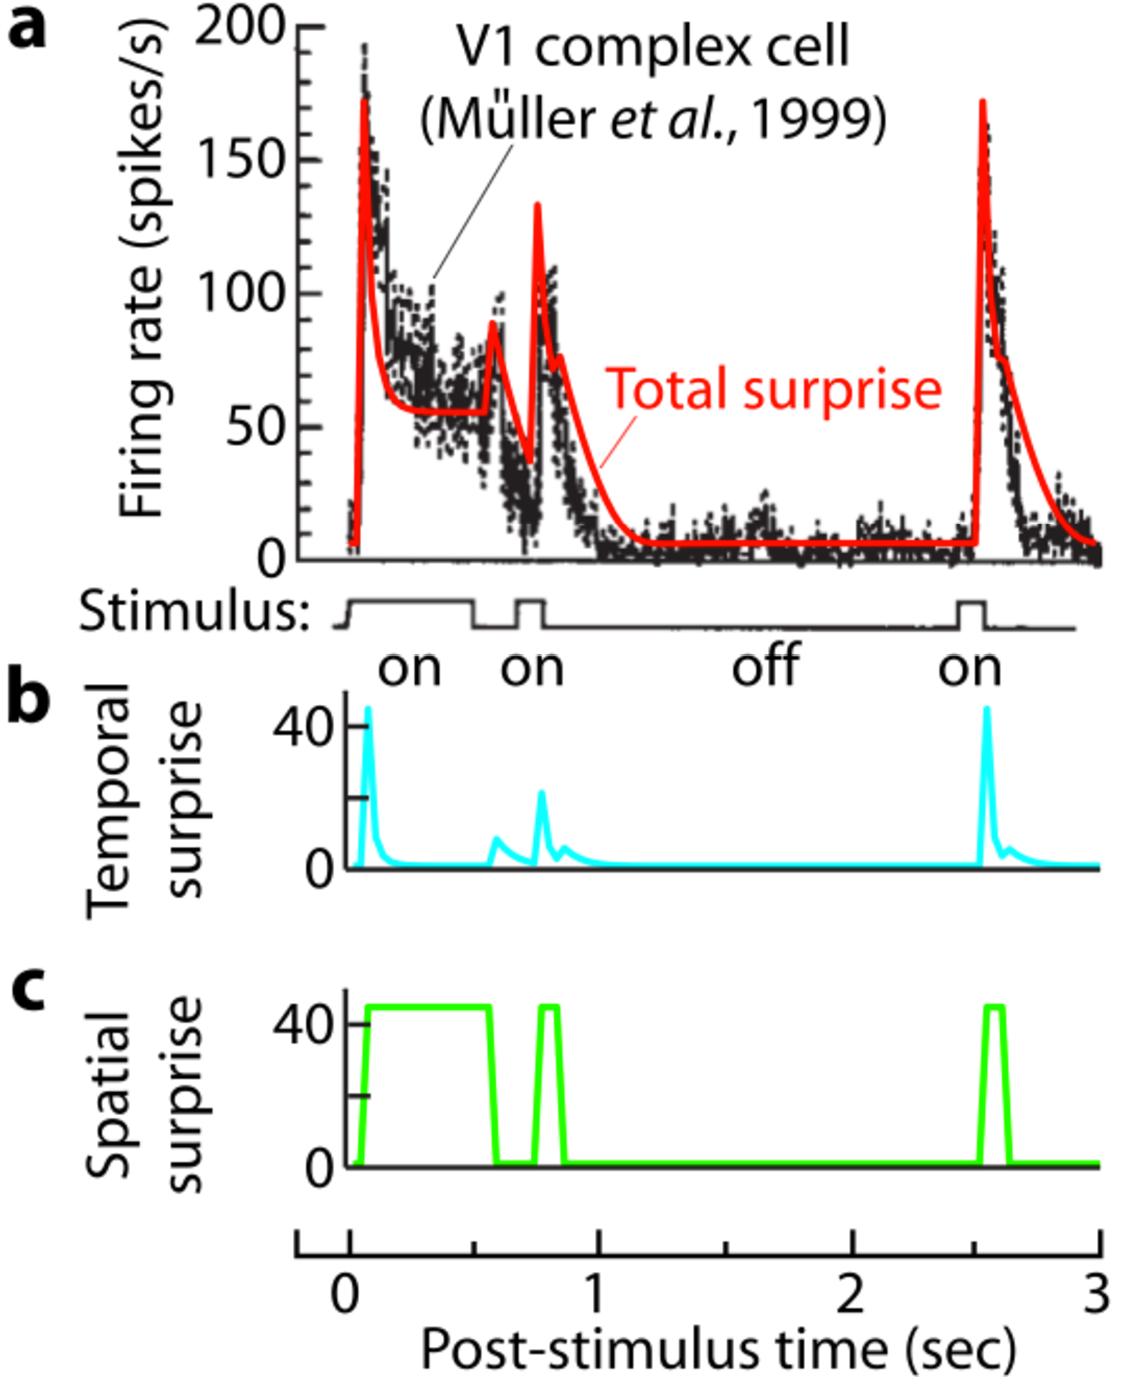
\includegraphics[width=0.4\textwidth]{../../figures/surprise-ittibaldi}
	\end{center}
\end{frame}


\begin{frame}{Surprise theory}
	\begin{itemize}
		\item Adaptation to sensors:
		\begin{itemize}
			\item Owen Langman's M.S. thesis - UW Limnology, 2009
		\end{itemize}
		\item Uses identical surprise model (Gamma-Poisson) as Itti and Baldi
	\end{itemize}
\end{frame}


\begin{frame}{Surprise theory}
	\begin{itemize}
		\item Problems with original theory:
		\begin{itemize}
			\item Ad-hoc ``memory" parameter must be tuned manually
			\item Cannot track mean and variance simultaneously
			\item Technically only applicable to discrete data (e.g. counts)
		\end{itemize}
	\end{itemize}
\end{frame}


\subsection{Bayesian statistics}


\begin{frame}{Bayesian statistics}
	Bayesian statistics views a probability distribution as representing our degree of belief. This idea can be applied both to our data and to the underlying data-generating model.\\
	\vspace{3mm}
	\begin{itemize}
		\item Examples of the three distributions used in this work:
		\begin{itemize}
			\item $X \sim \text{Normal}(\mu=0, \tau=1)$
			\item $Y \sim \text{Gamma}(\alpha=2, \beta=1)$
			\item $Z \sim \text{t}_{\nu=4}(\mu=0, \sigma^2=1)$
		\end{itemize}
	\end{itemize}
	\begin{center}
		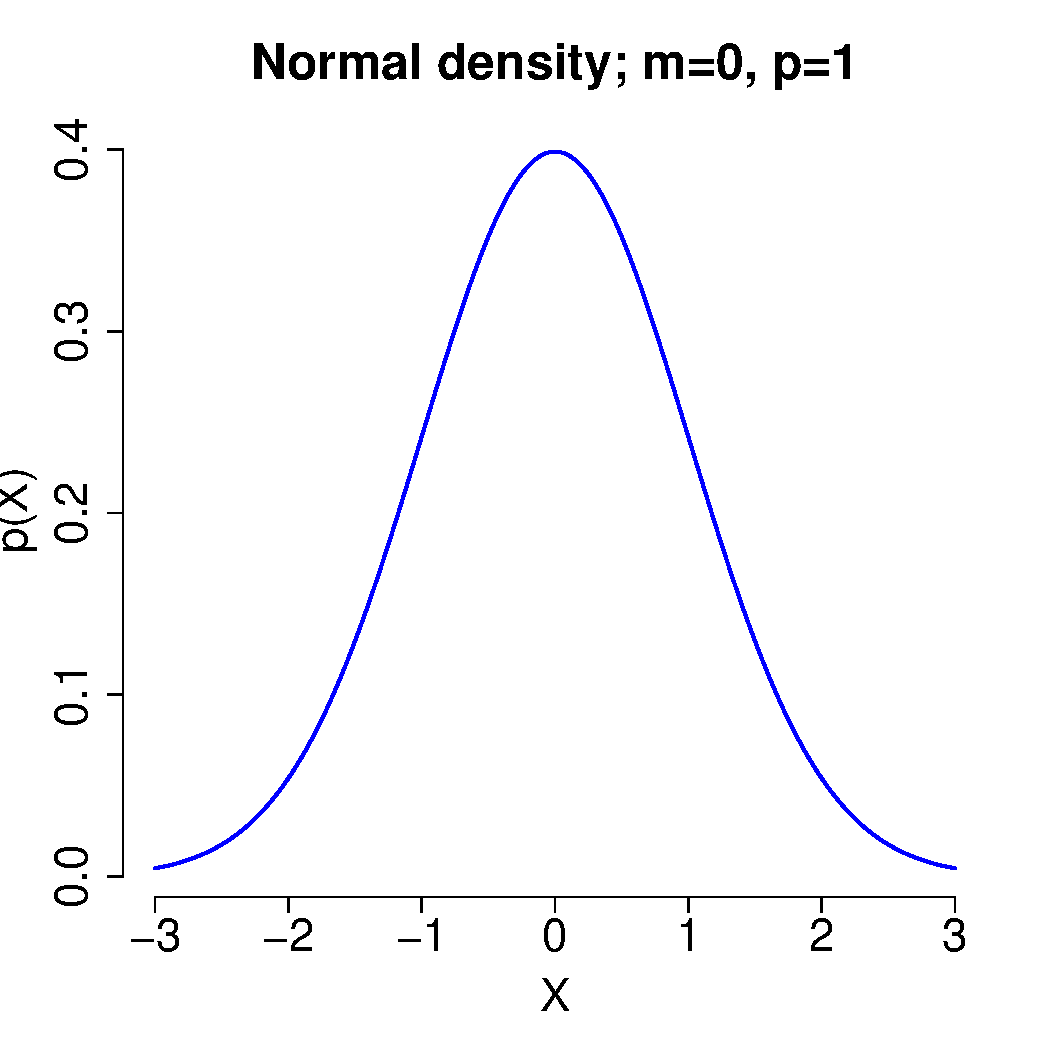
\includegraphics[width=0.33\textwidth]{../../figures/normal_pdf}
		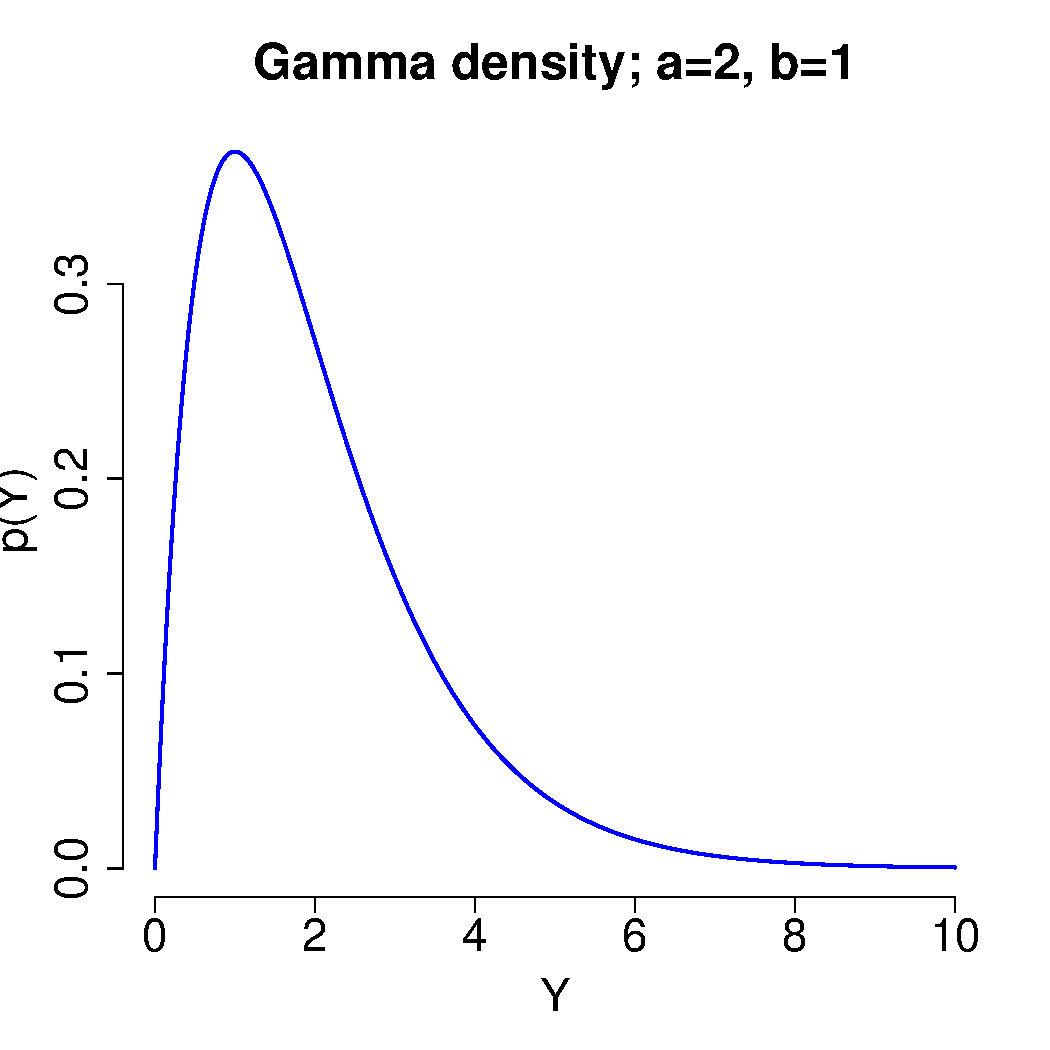
\includegraphics[width=0.33\textwidth]{../../figures/gamma_pdf}
		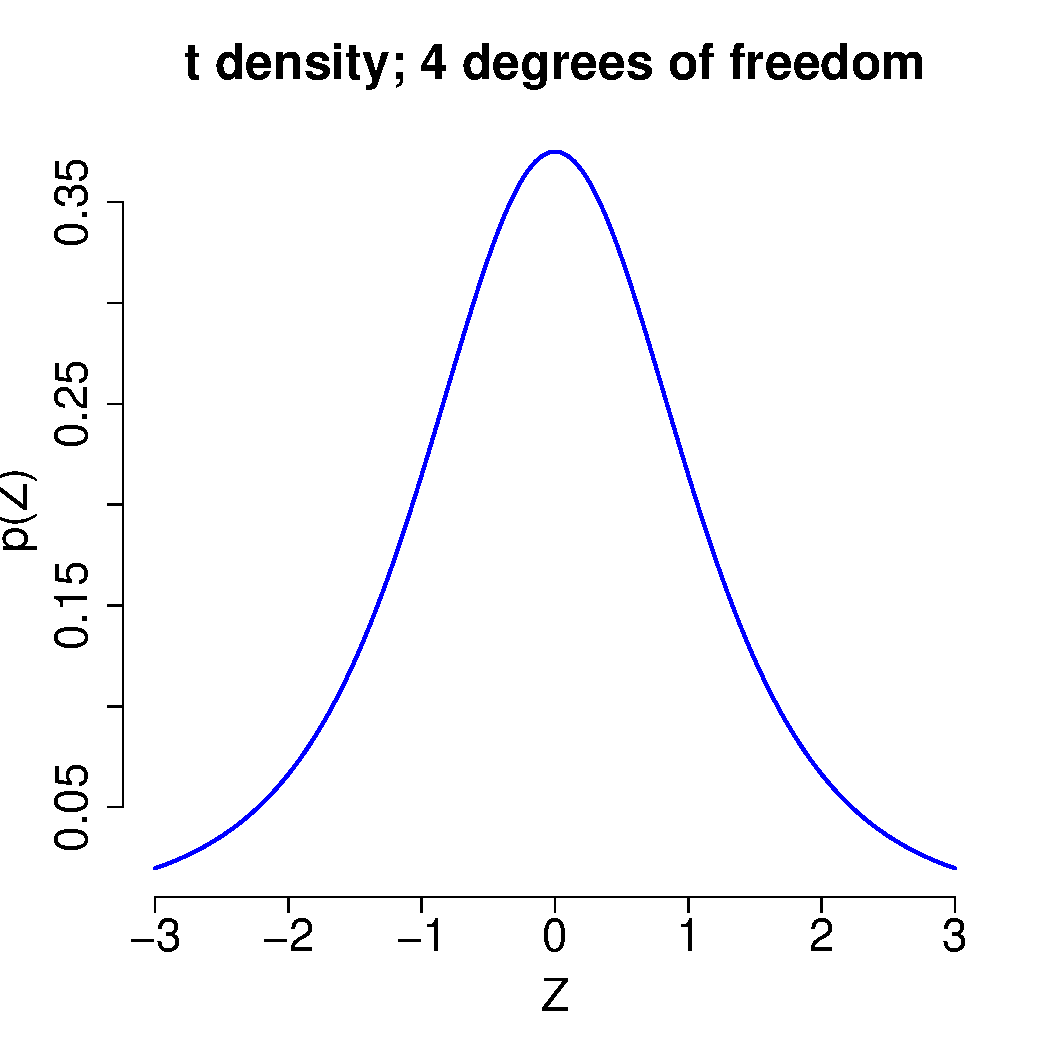
\includegraphics[width=0.33\textwidth]{../../figures/t_pdf}
	\end{center}
\end{frame}


\begin{frame}{Hierarchical models}
	\begin{itemize}
		\item \visible<1->{A hierarchical model has more than one random element}
		\item \visible<1->{Randomness at one level feeds into the next}
	\end{itemize}
	\visible<2->{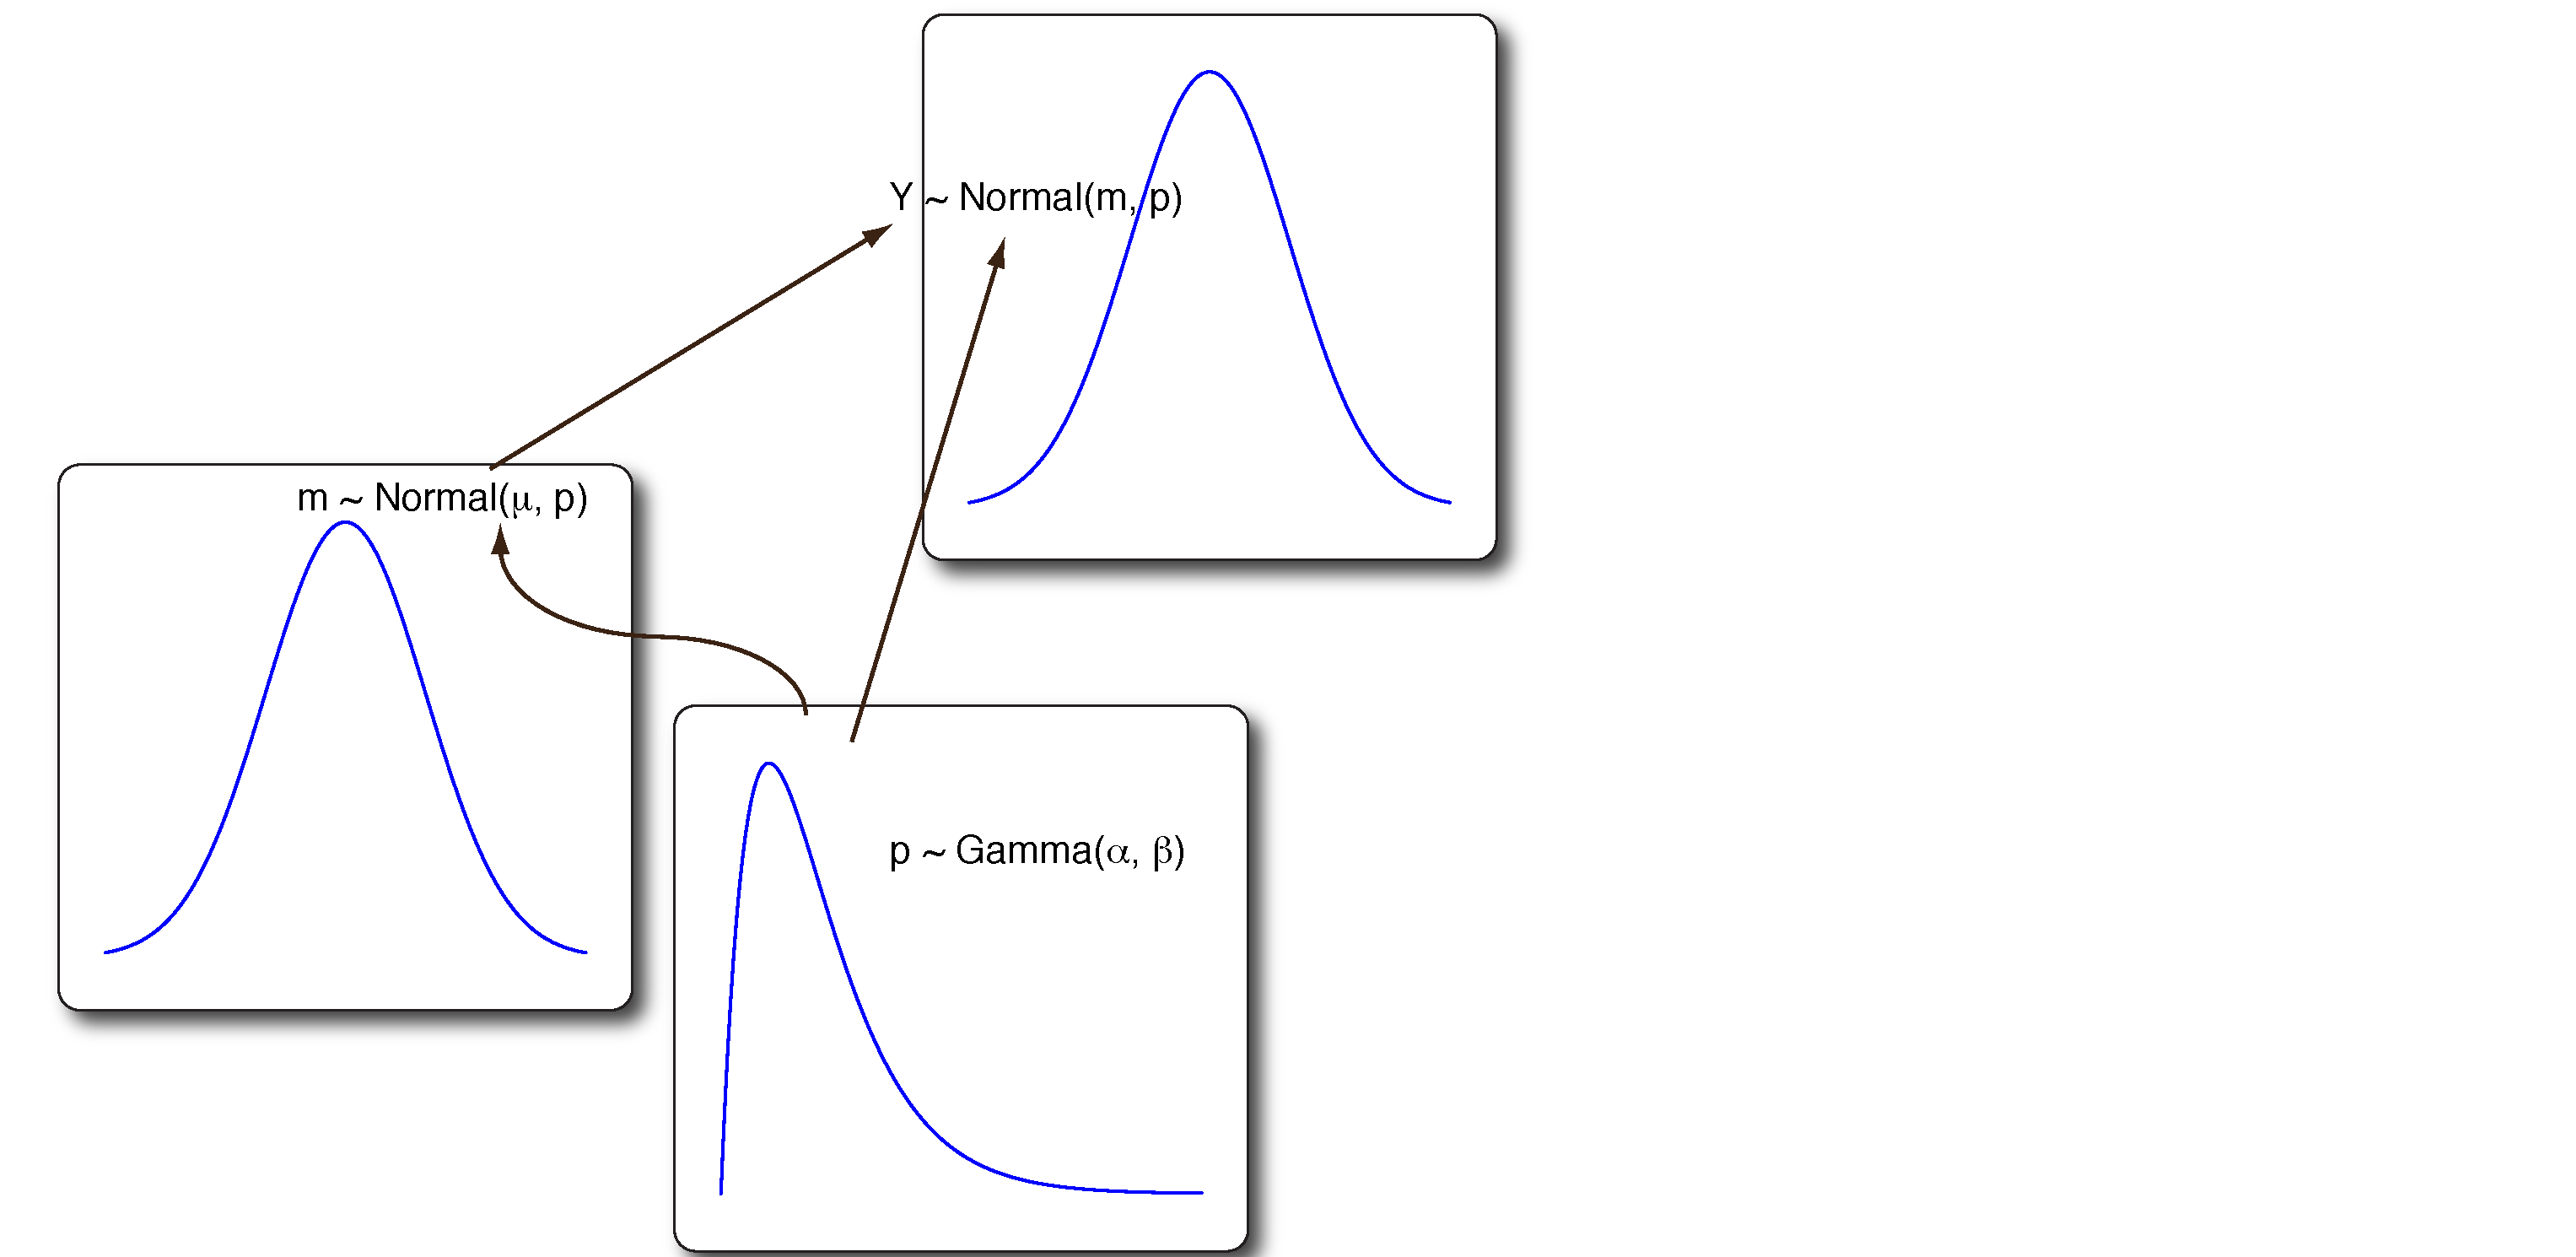
\includegraphics[width=\textwidth]{../../figures/hierarchical}}
\end{frame}


\begin{frame}{Hierarchical models}
	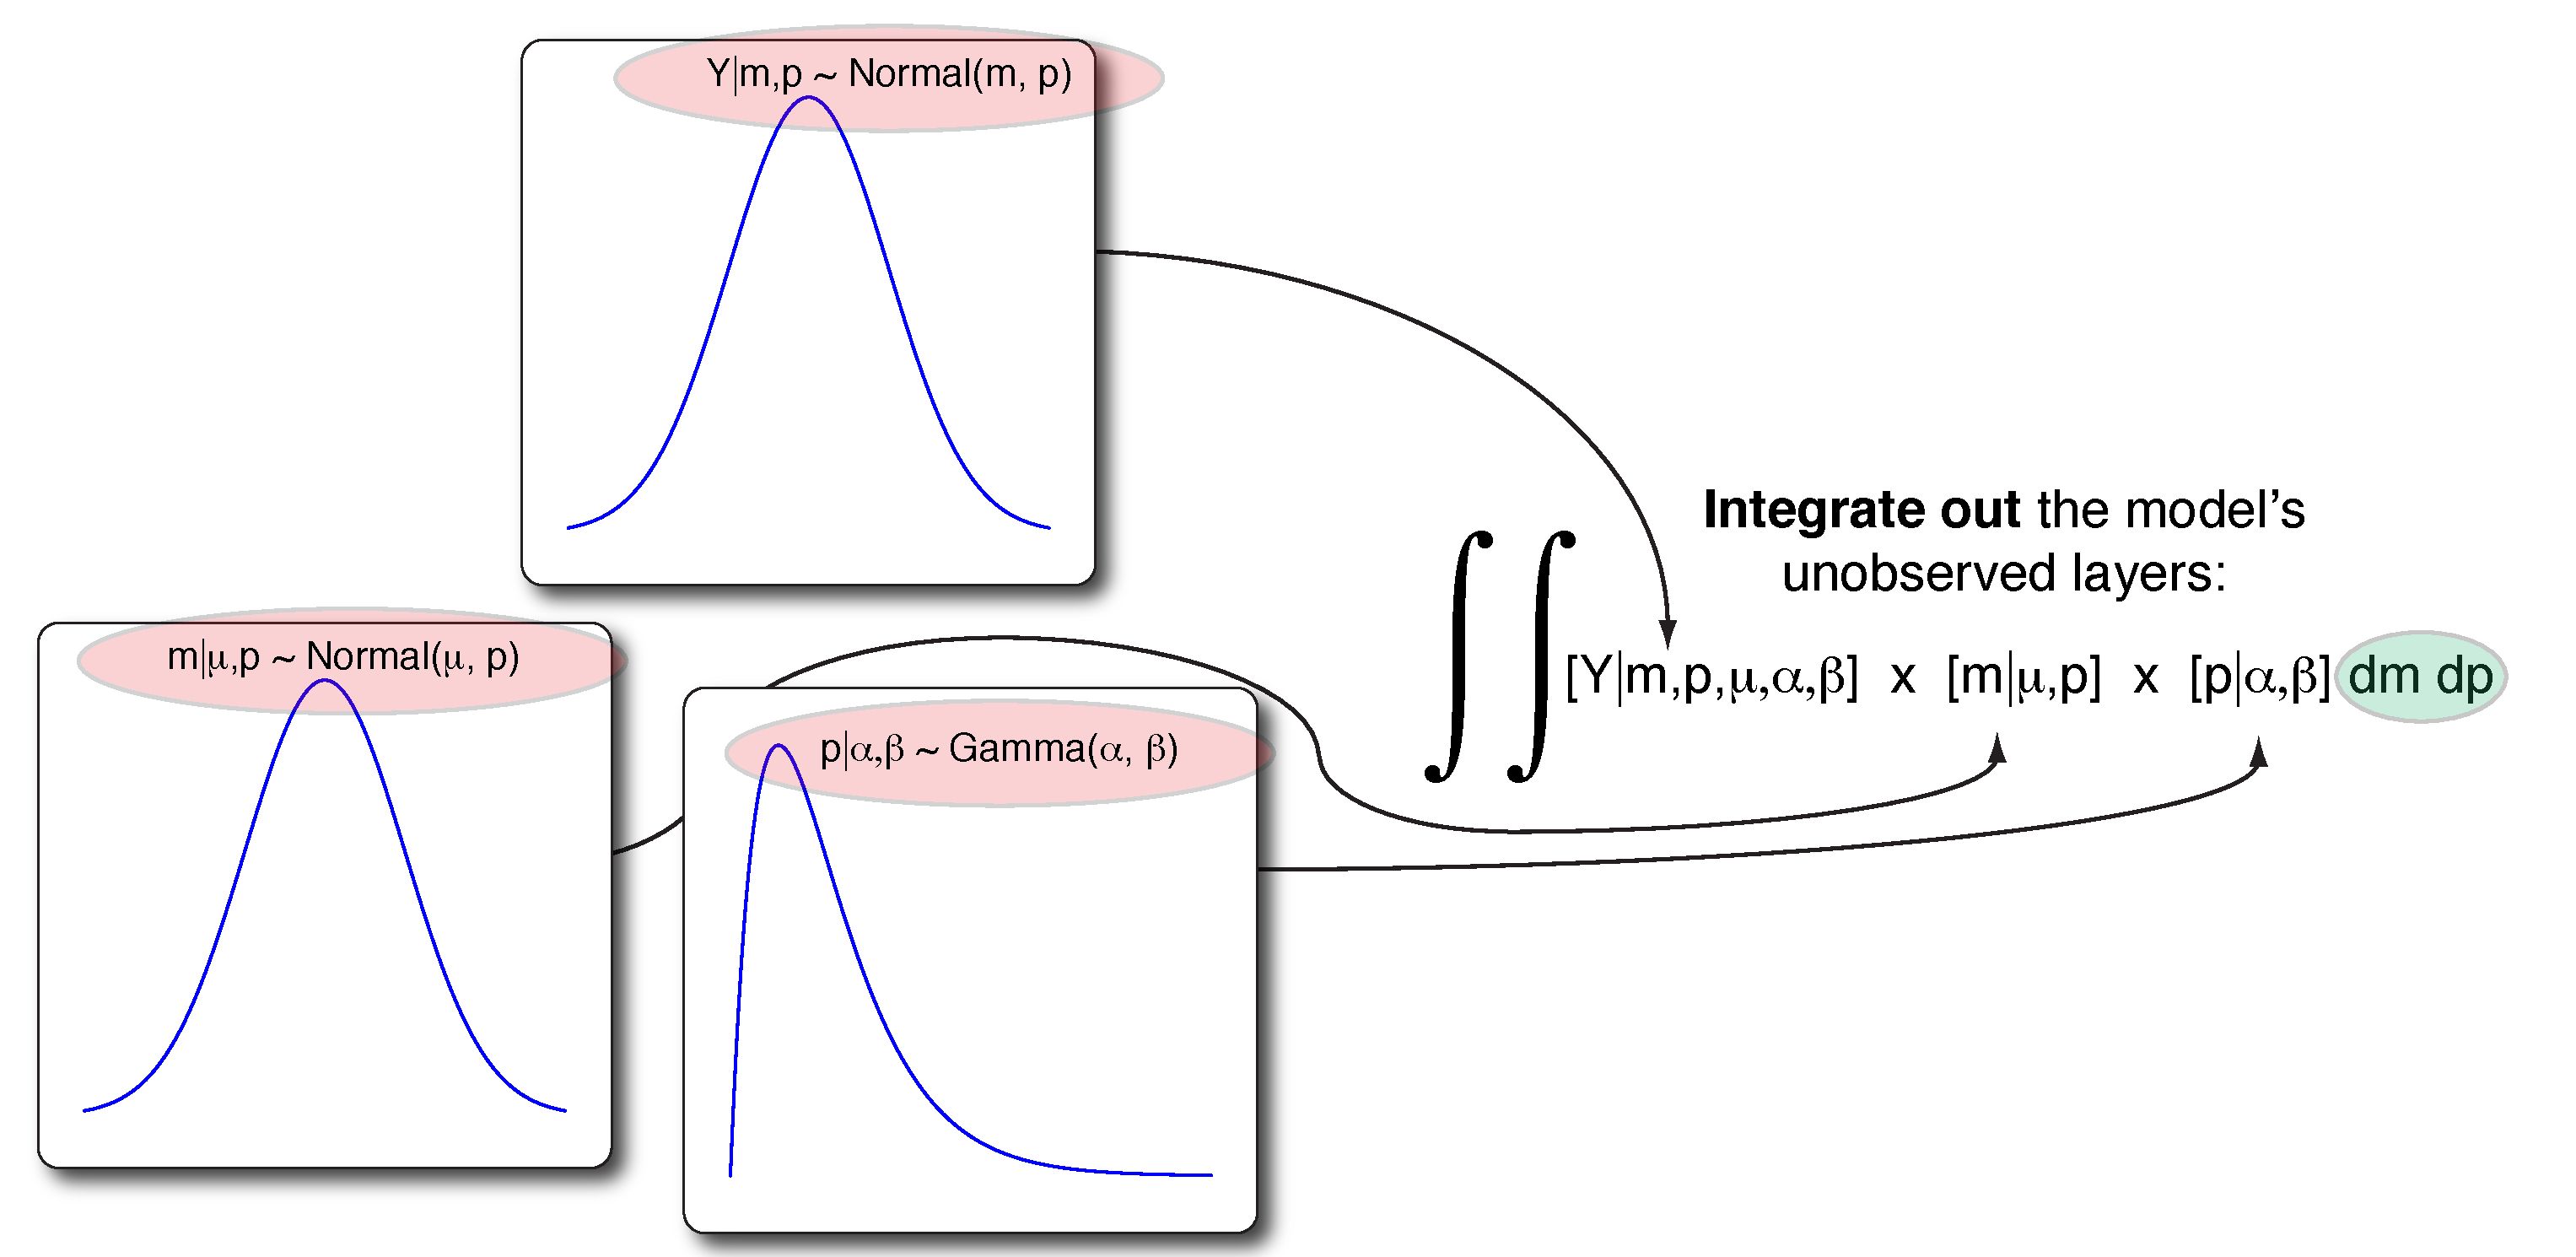
\includegraphics[width=\textwidth]{../../figures/hierarchical-integrate}
\end{frame}


\begin{frame}{Hierarchical models}
	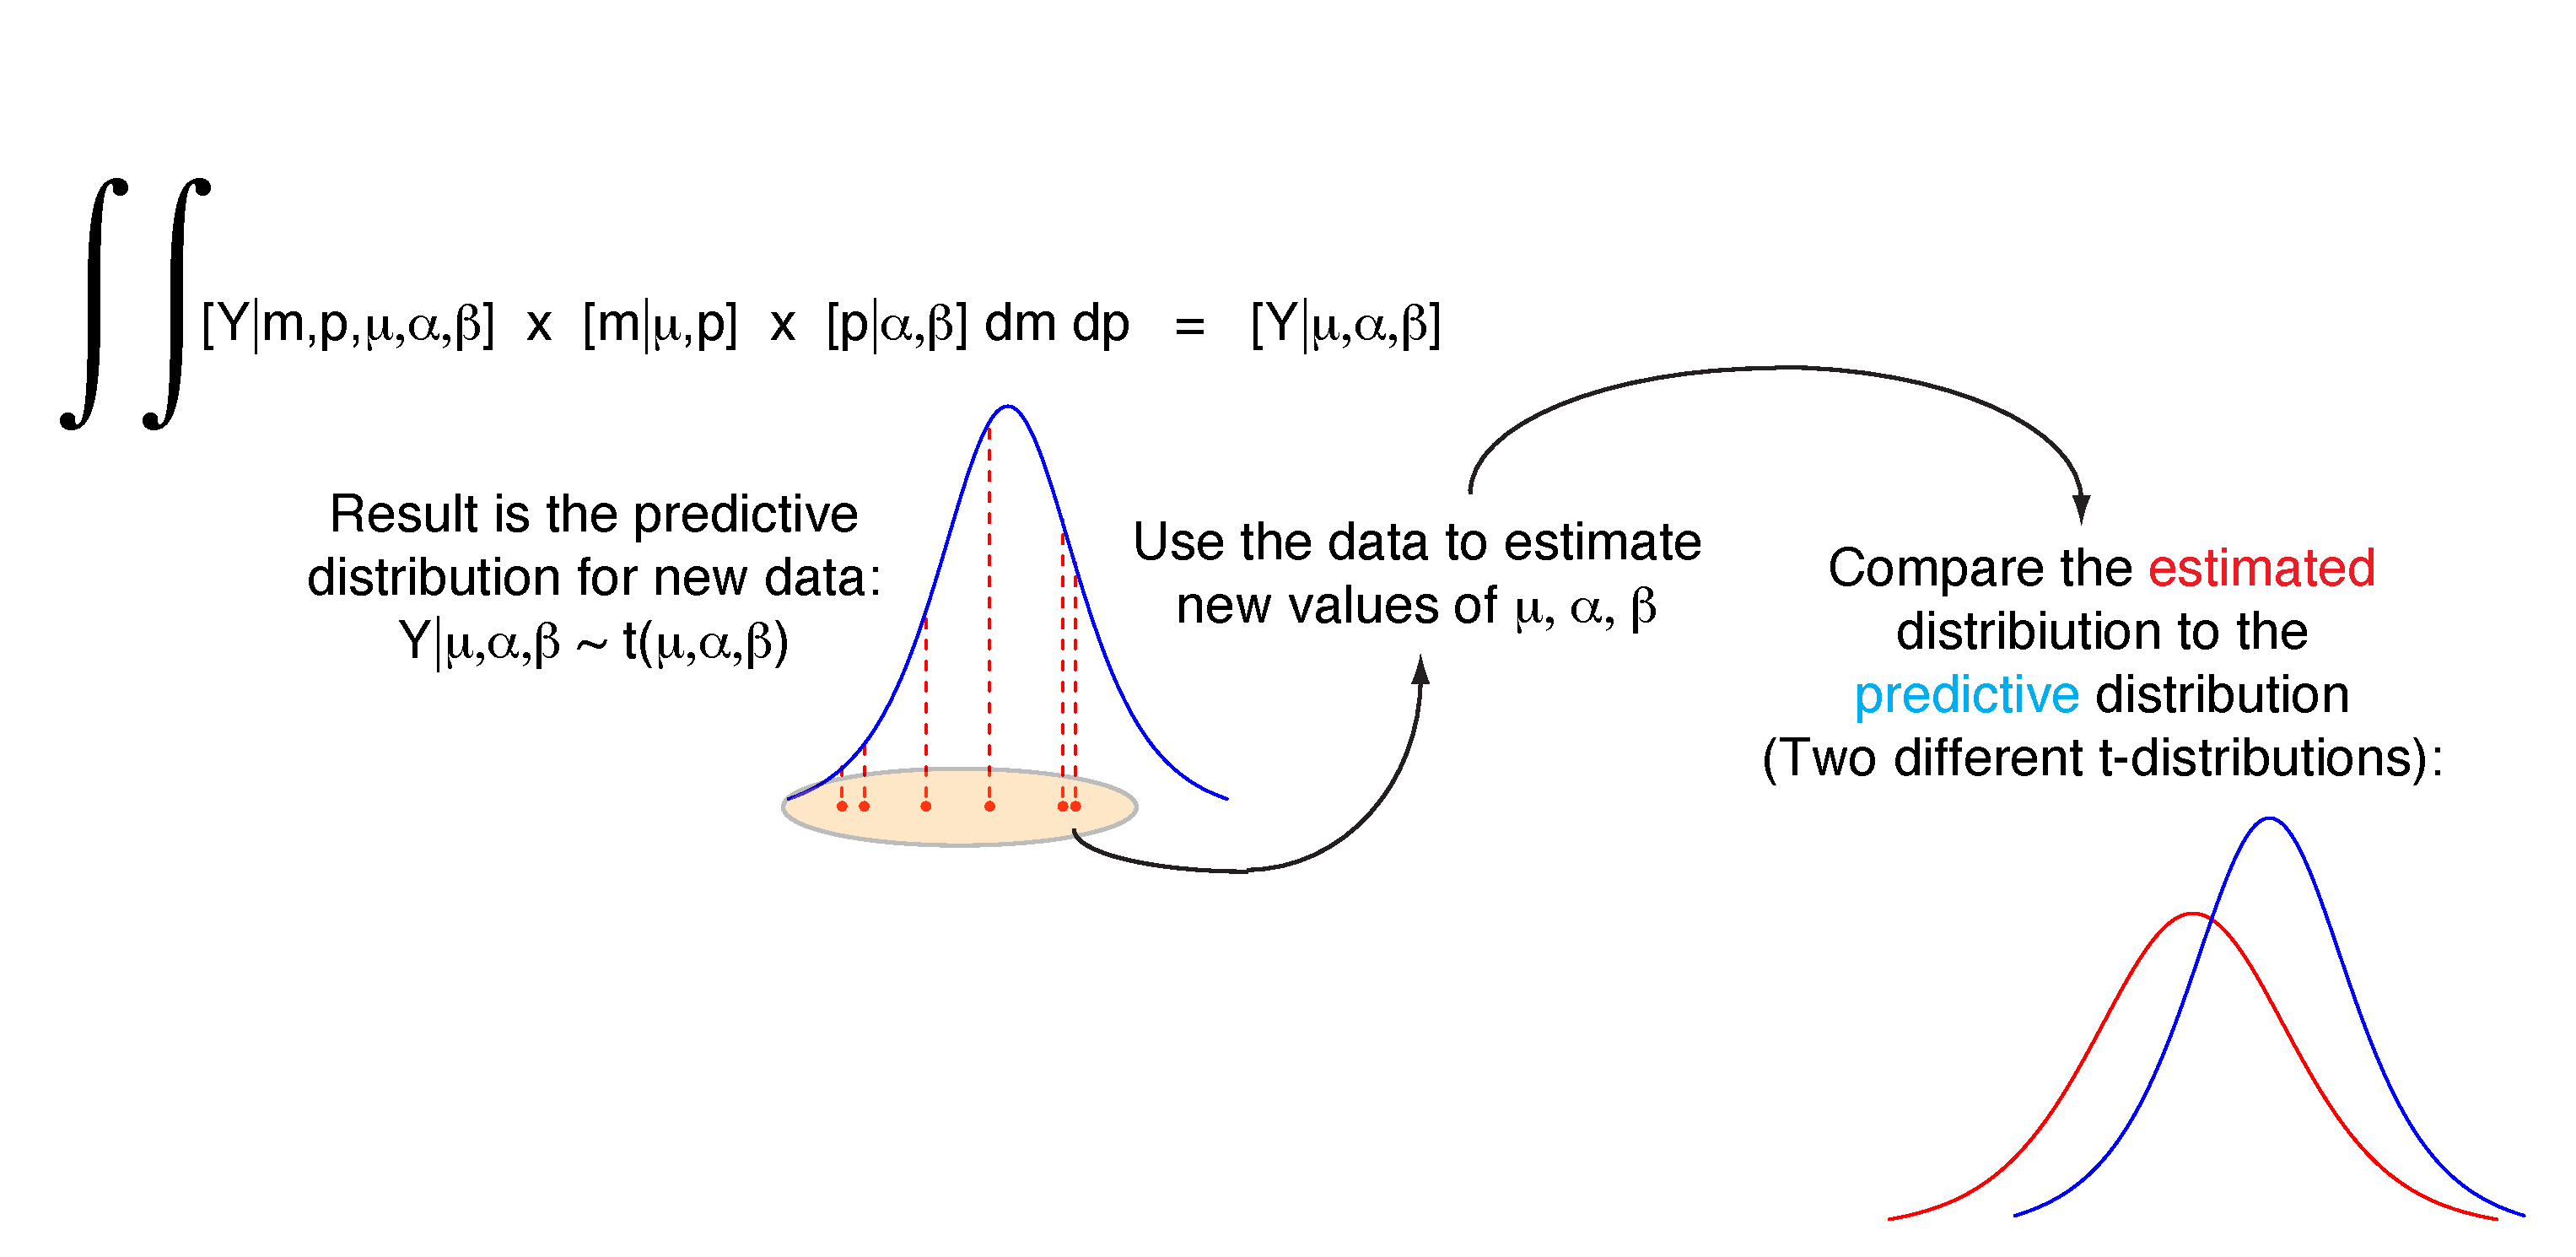
\includegraphics[width=\textwidth]{../../figures/hierarchical-marginal}
\end{frame}


\begin{frame}{Calculate the surprise}
	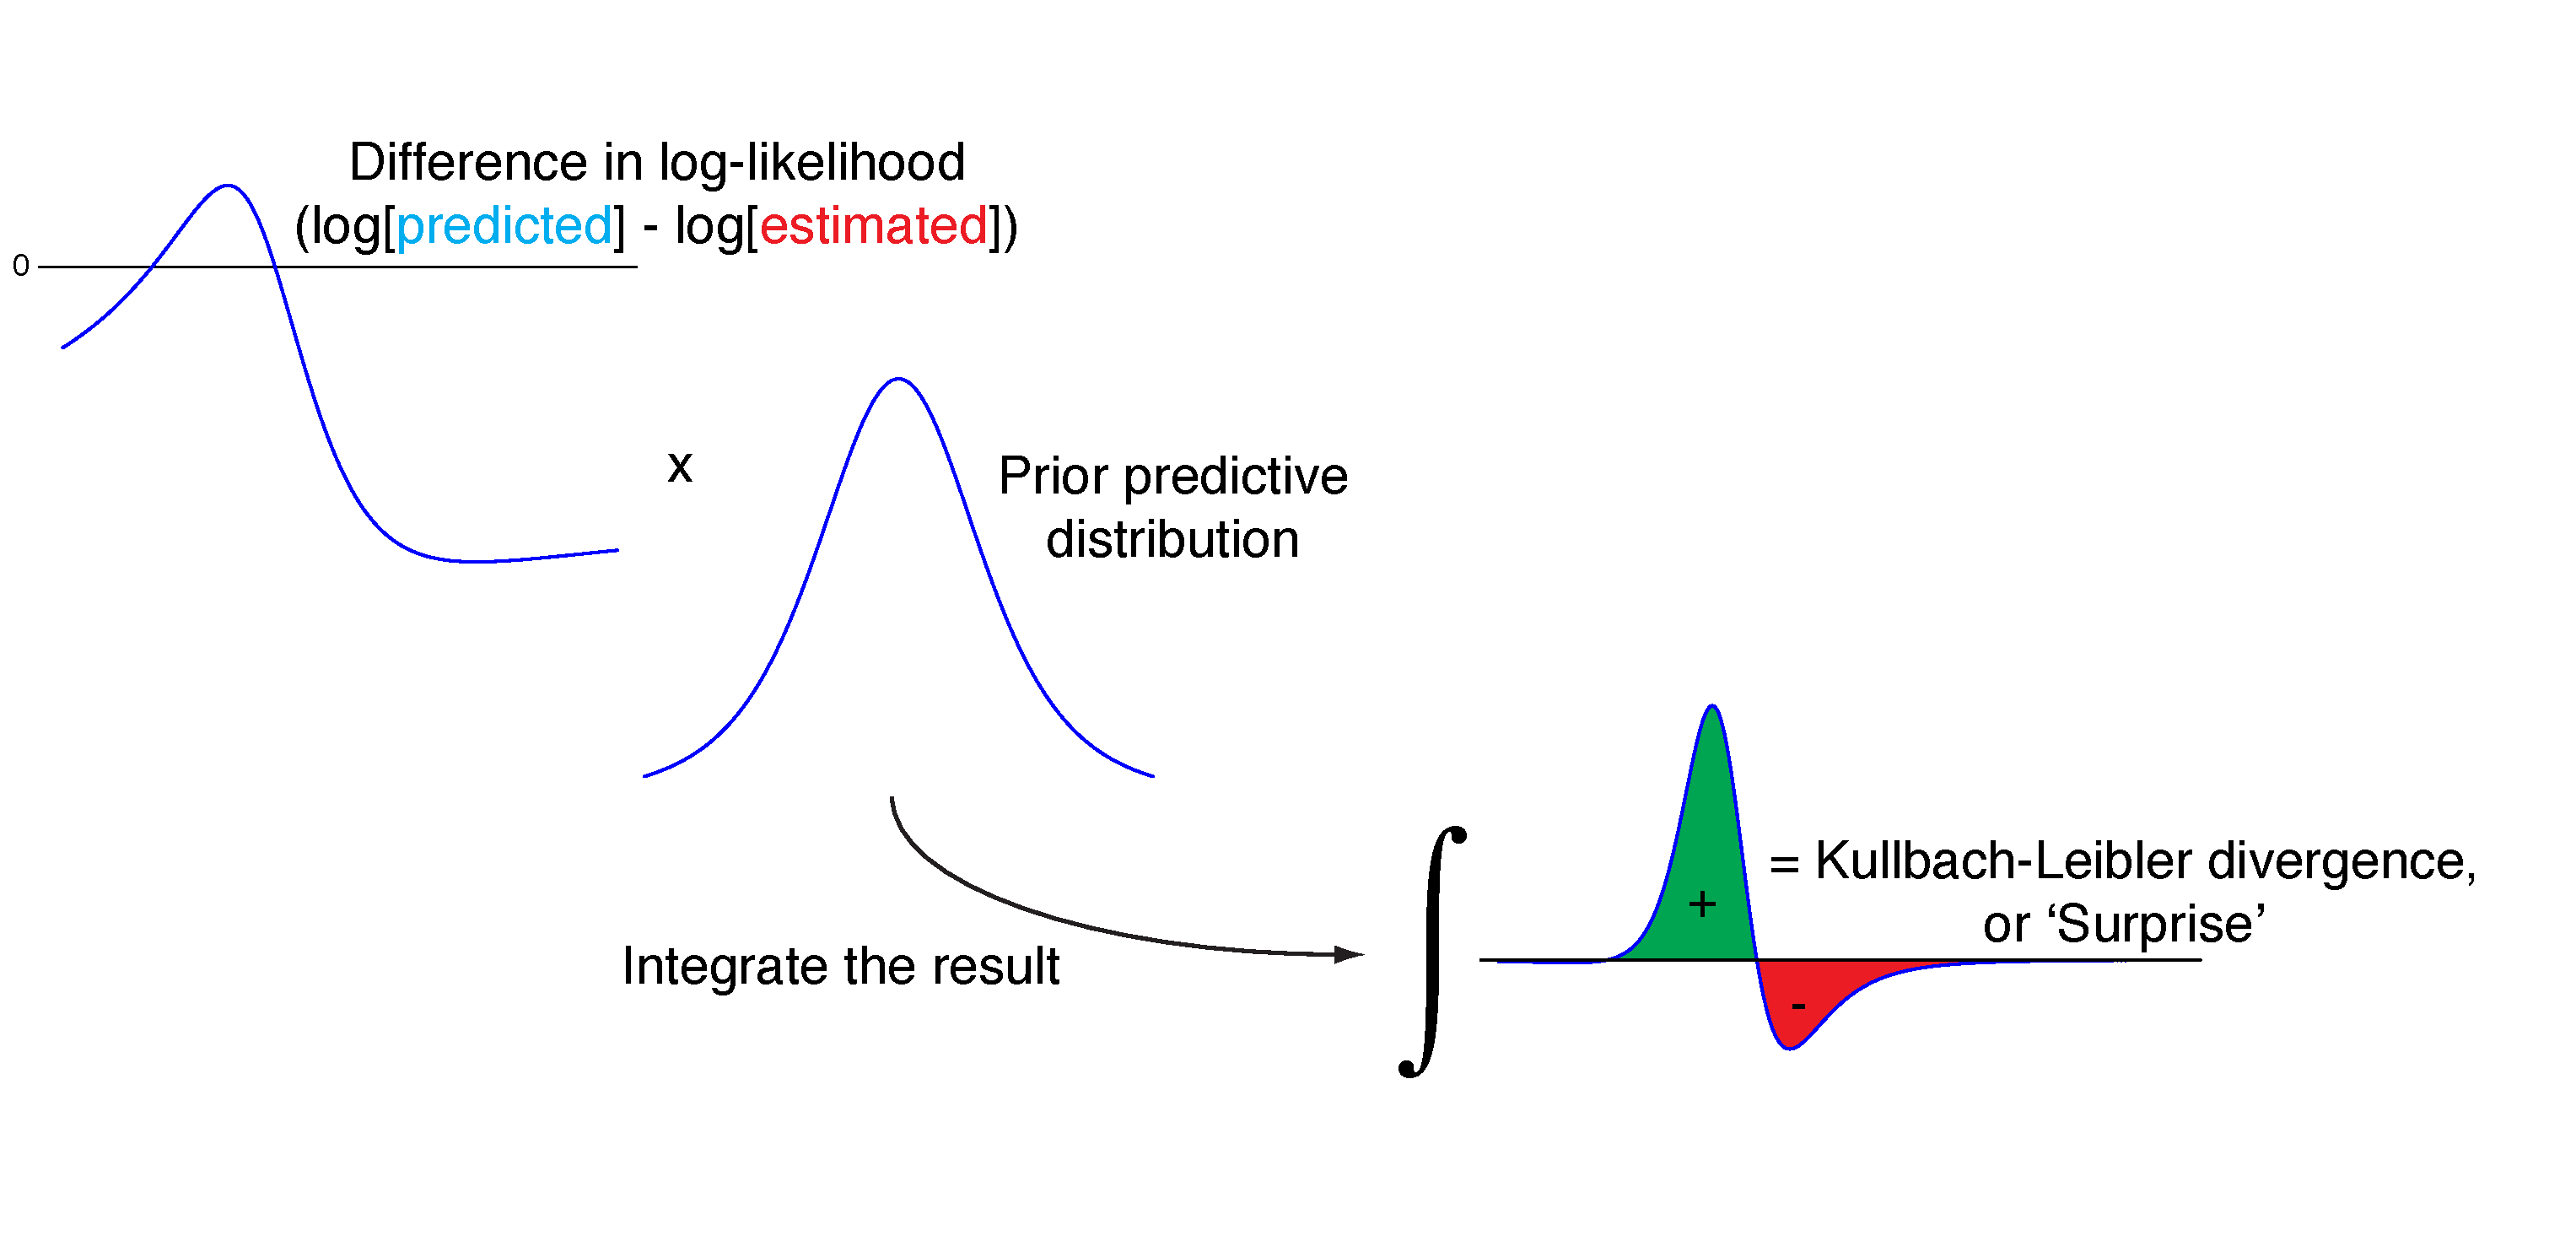
\includegraphics[width=\textwidth]{../../figures/hierarchical-surprise}
\end{frame}


\begin{frame}{Iterate the process}
	Use moving windows to iterate the process as new data comes in:
	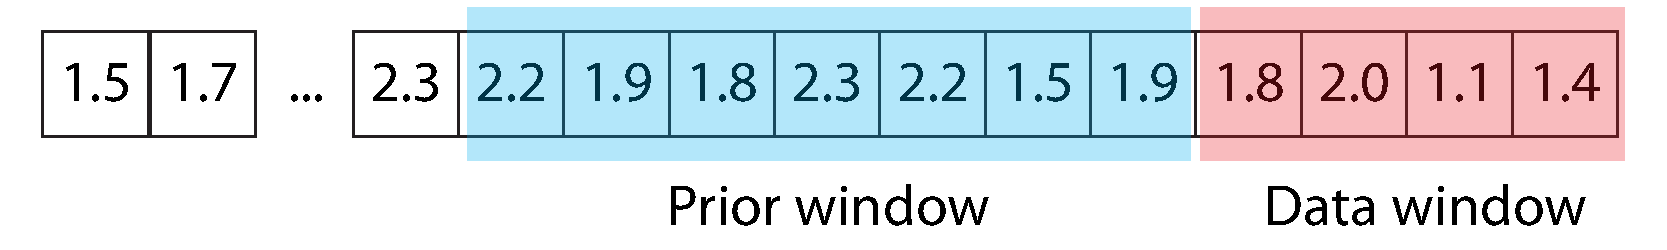
\includegraphics[width=\textwidth]{../../figures/data-window}
\end{frame}


\section{Examples}
\subsection{Simulations}
%Simulation study


\begin{frame}{Simulated surprise}
	Surprise generated by a sudden change in mean:
	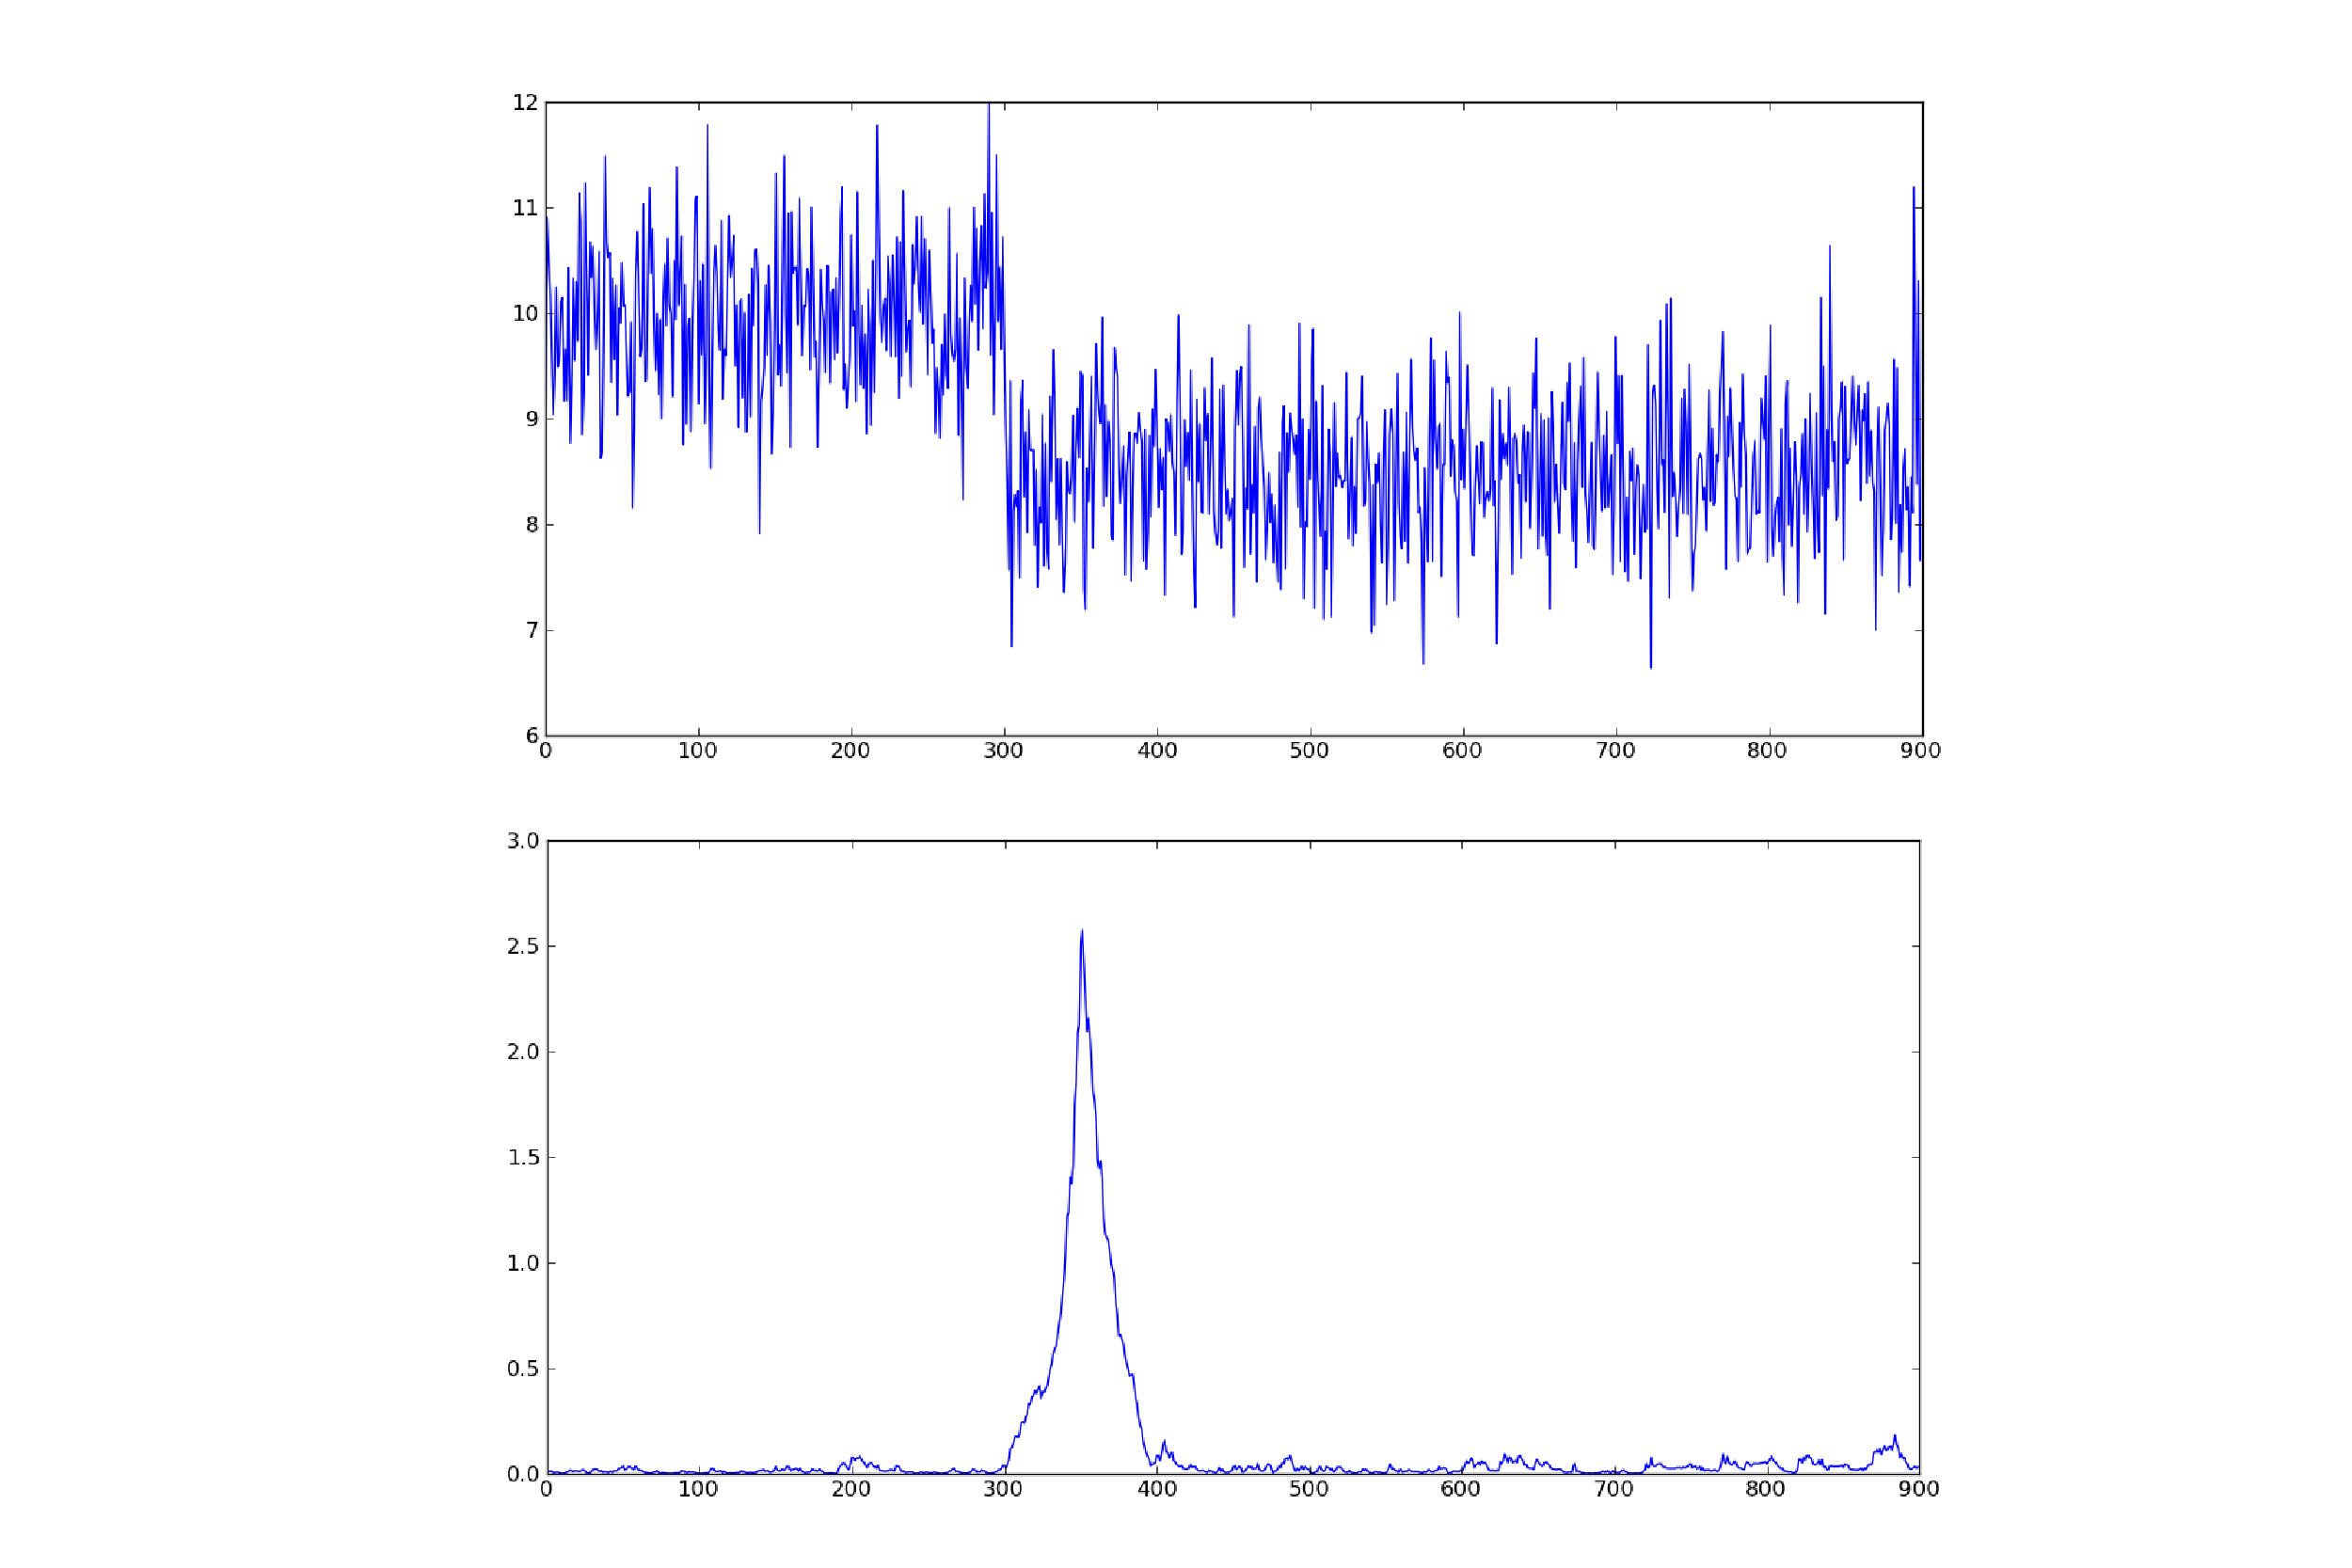
\includegraphics[width=\textwidth]{../../figures/mock1}
\end{frame}


\begin{frame}{Simulated surprise}
	Surprise generated by a sudden change in variance:
	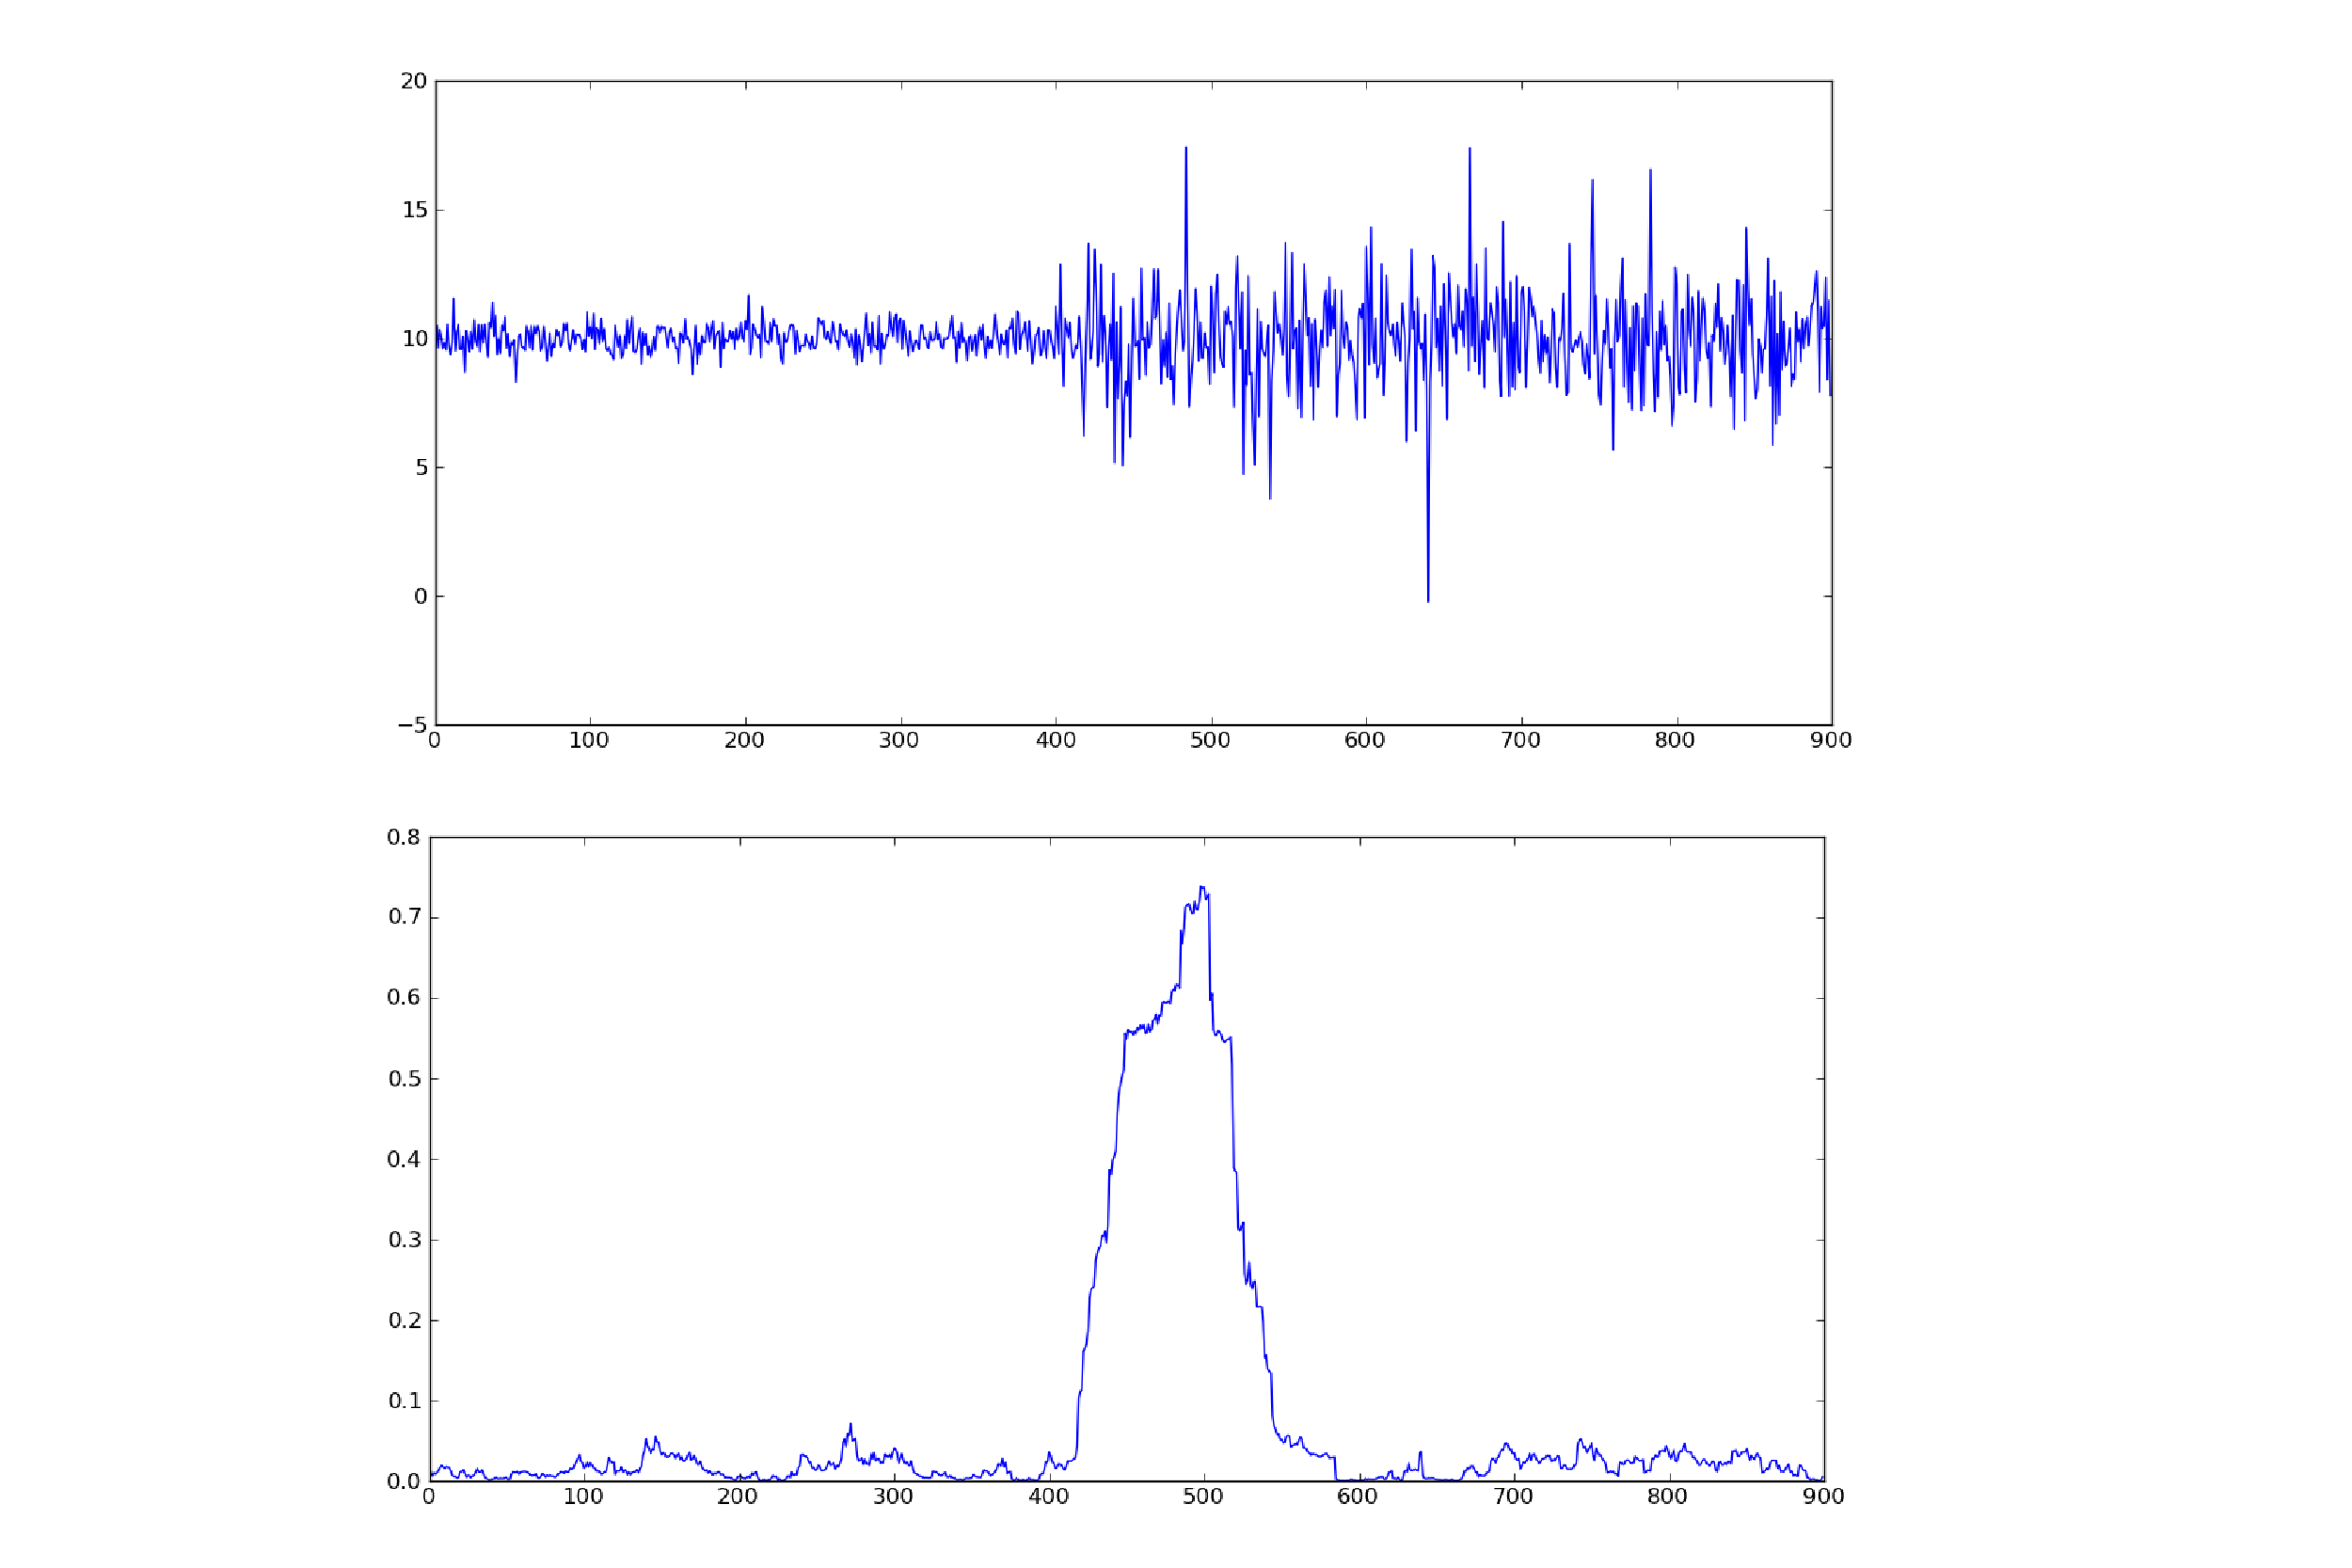
\includegraphics[width=\textwidth]{../../figures/mock3}
\end{frame}



\subsection{Field data}


\begin{frame}{Field data}
	Pheasant Branch (Middleton, WI) water temp (Dec 2011 - Jan 2012):
	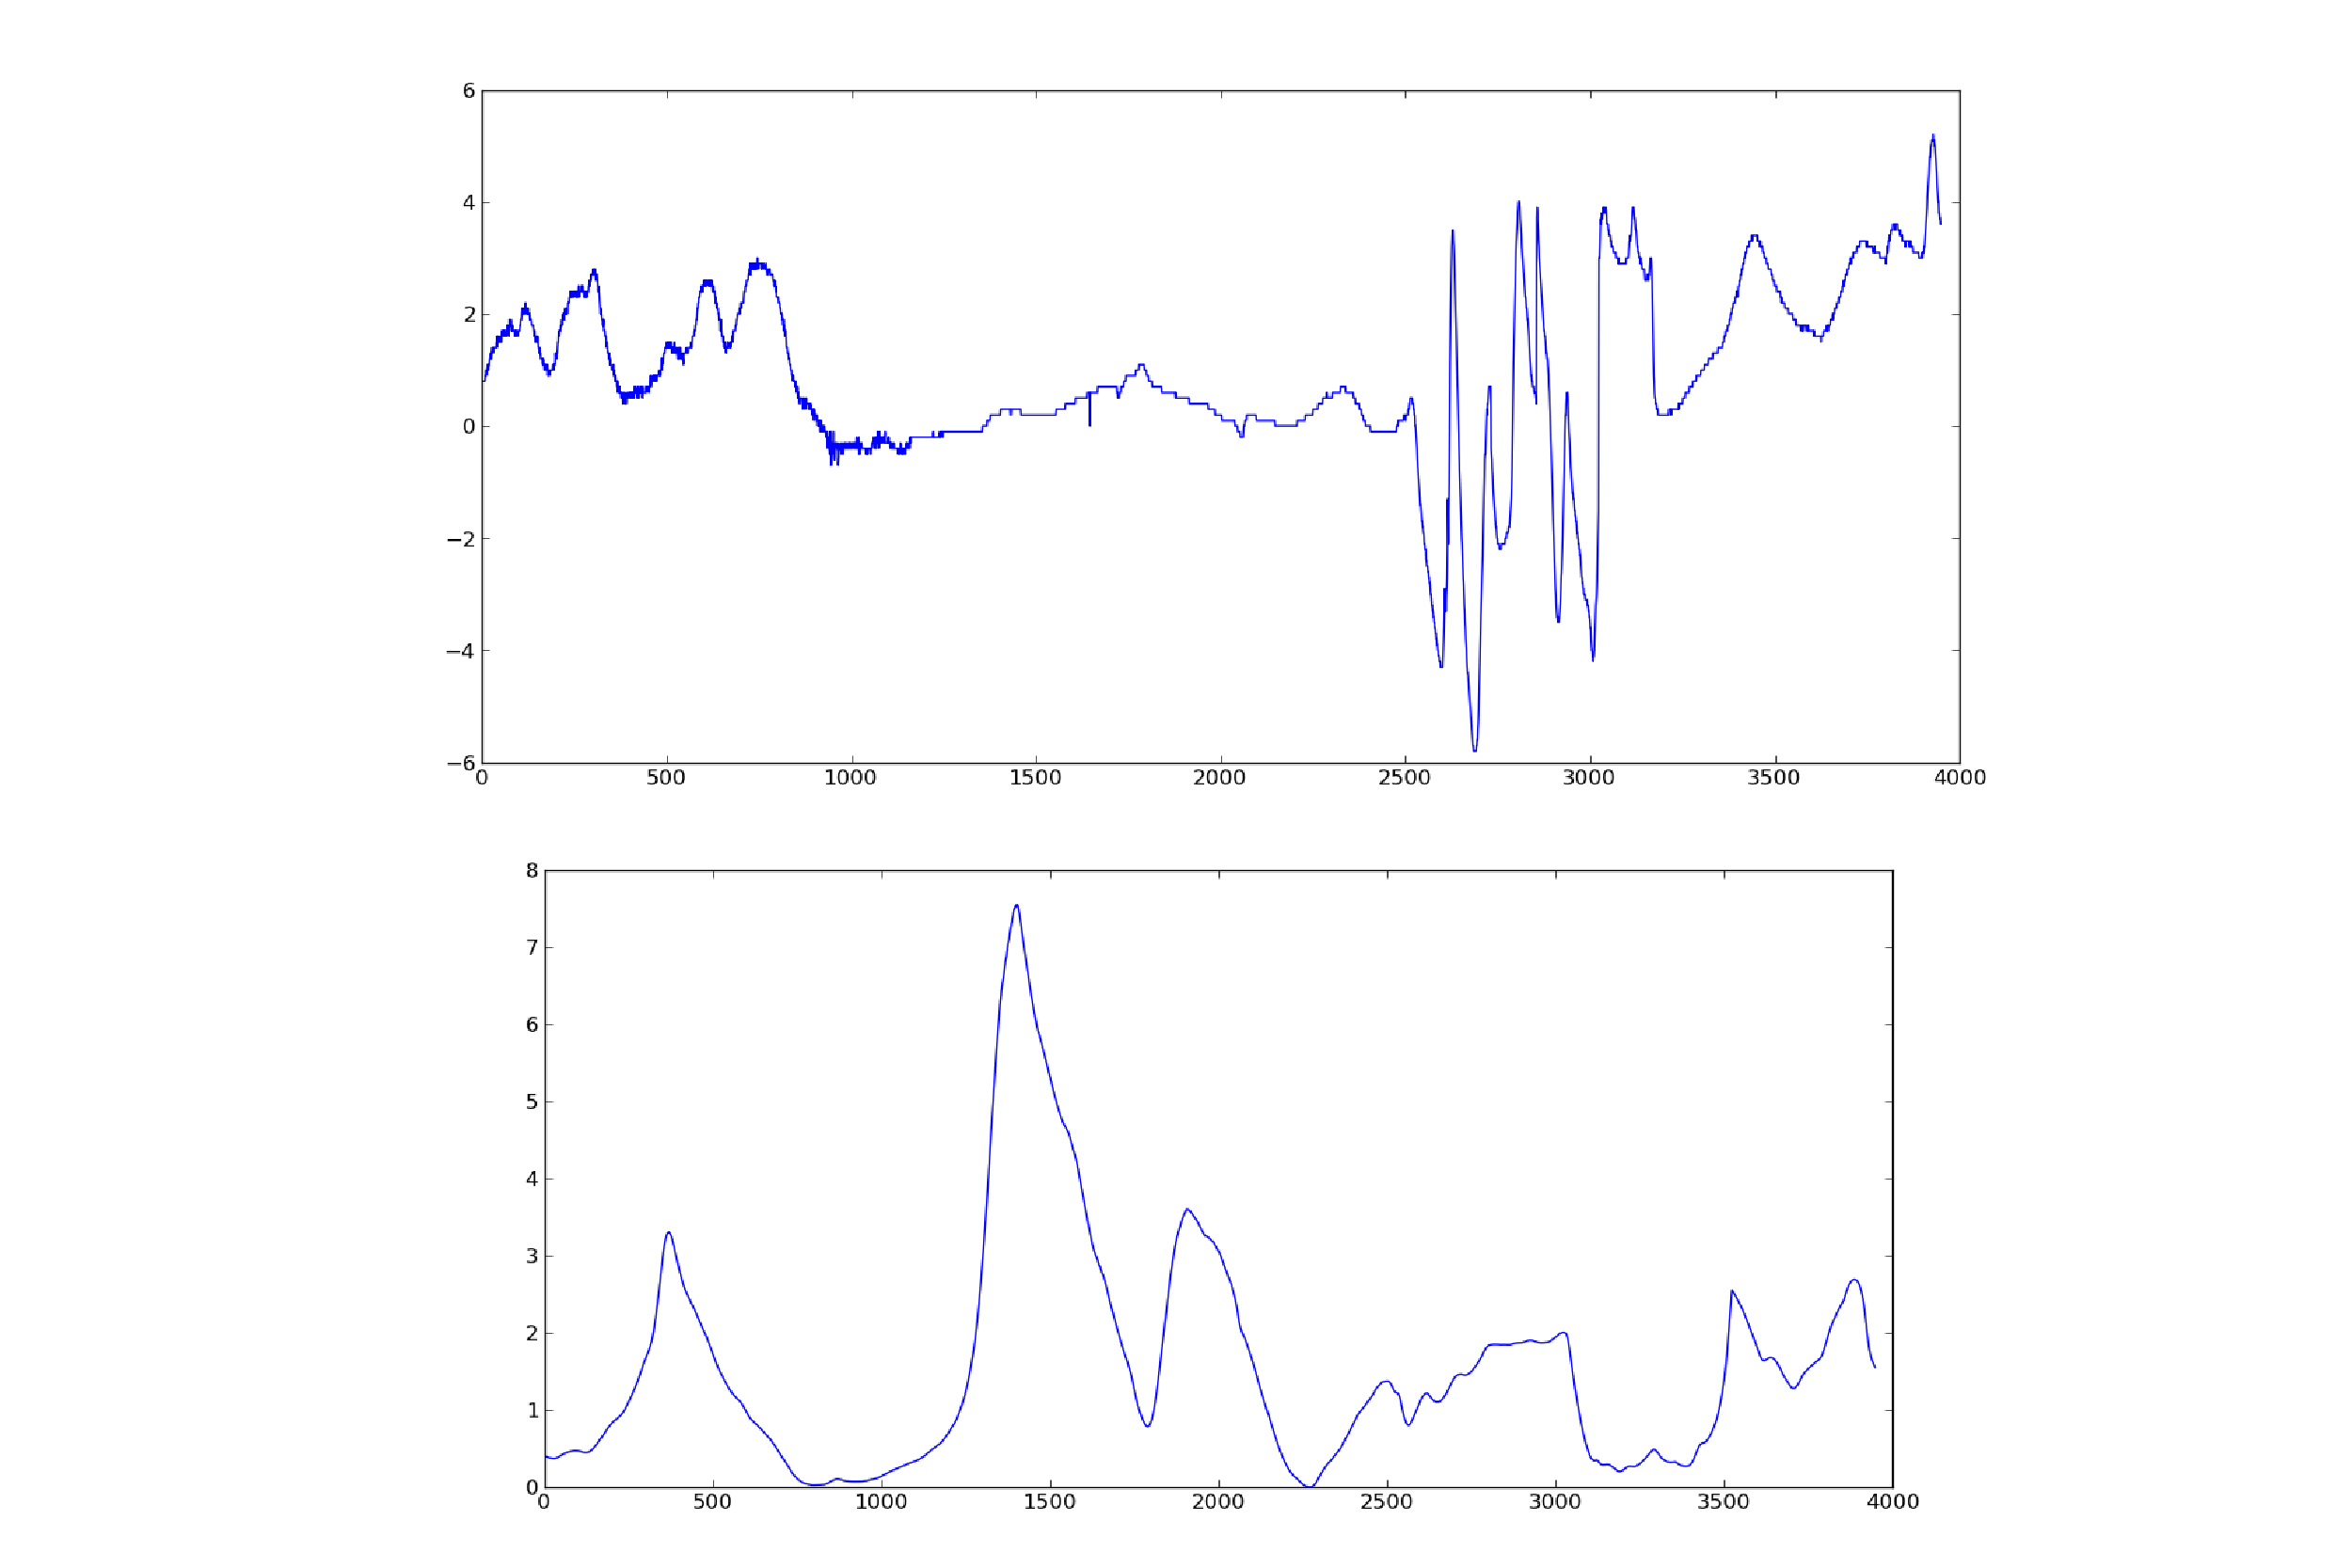
\includegraphics[width=\textwidth]{../../figures/pheasantbranch}
\end{frame}


\begin{frame}{Field data}
	Trout Lake LTER site (northern WI) CDOM (Nov. 2009):
	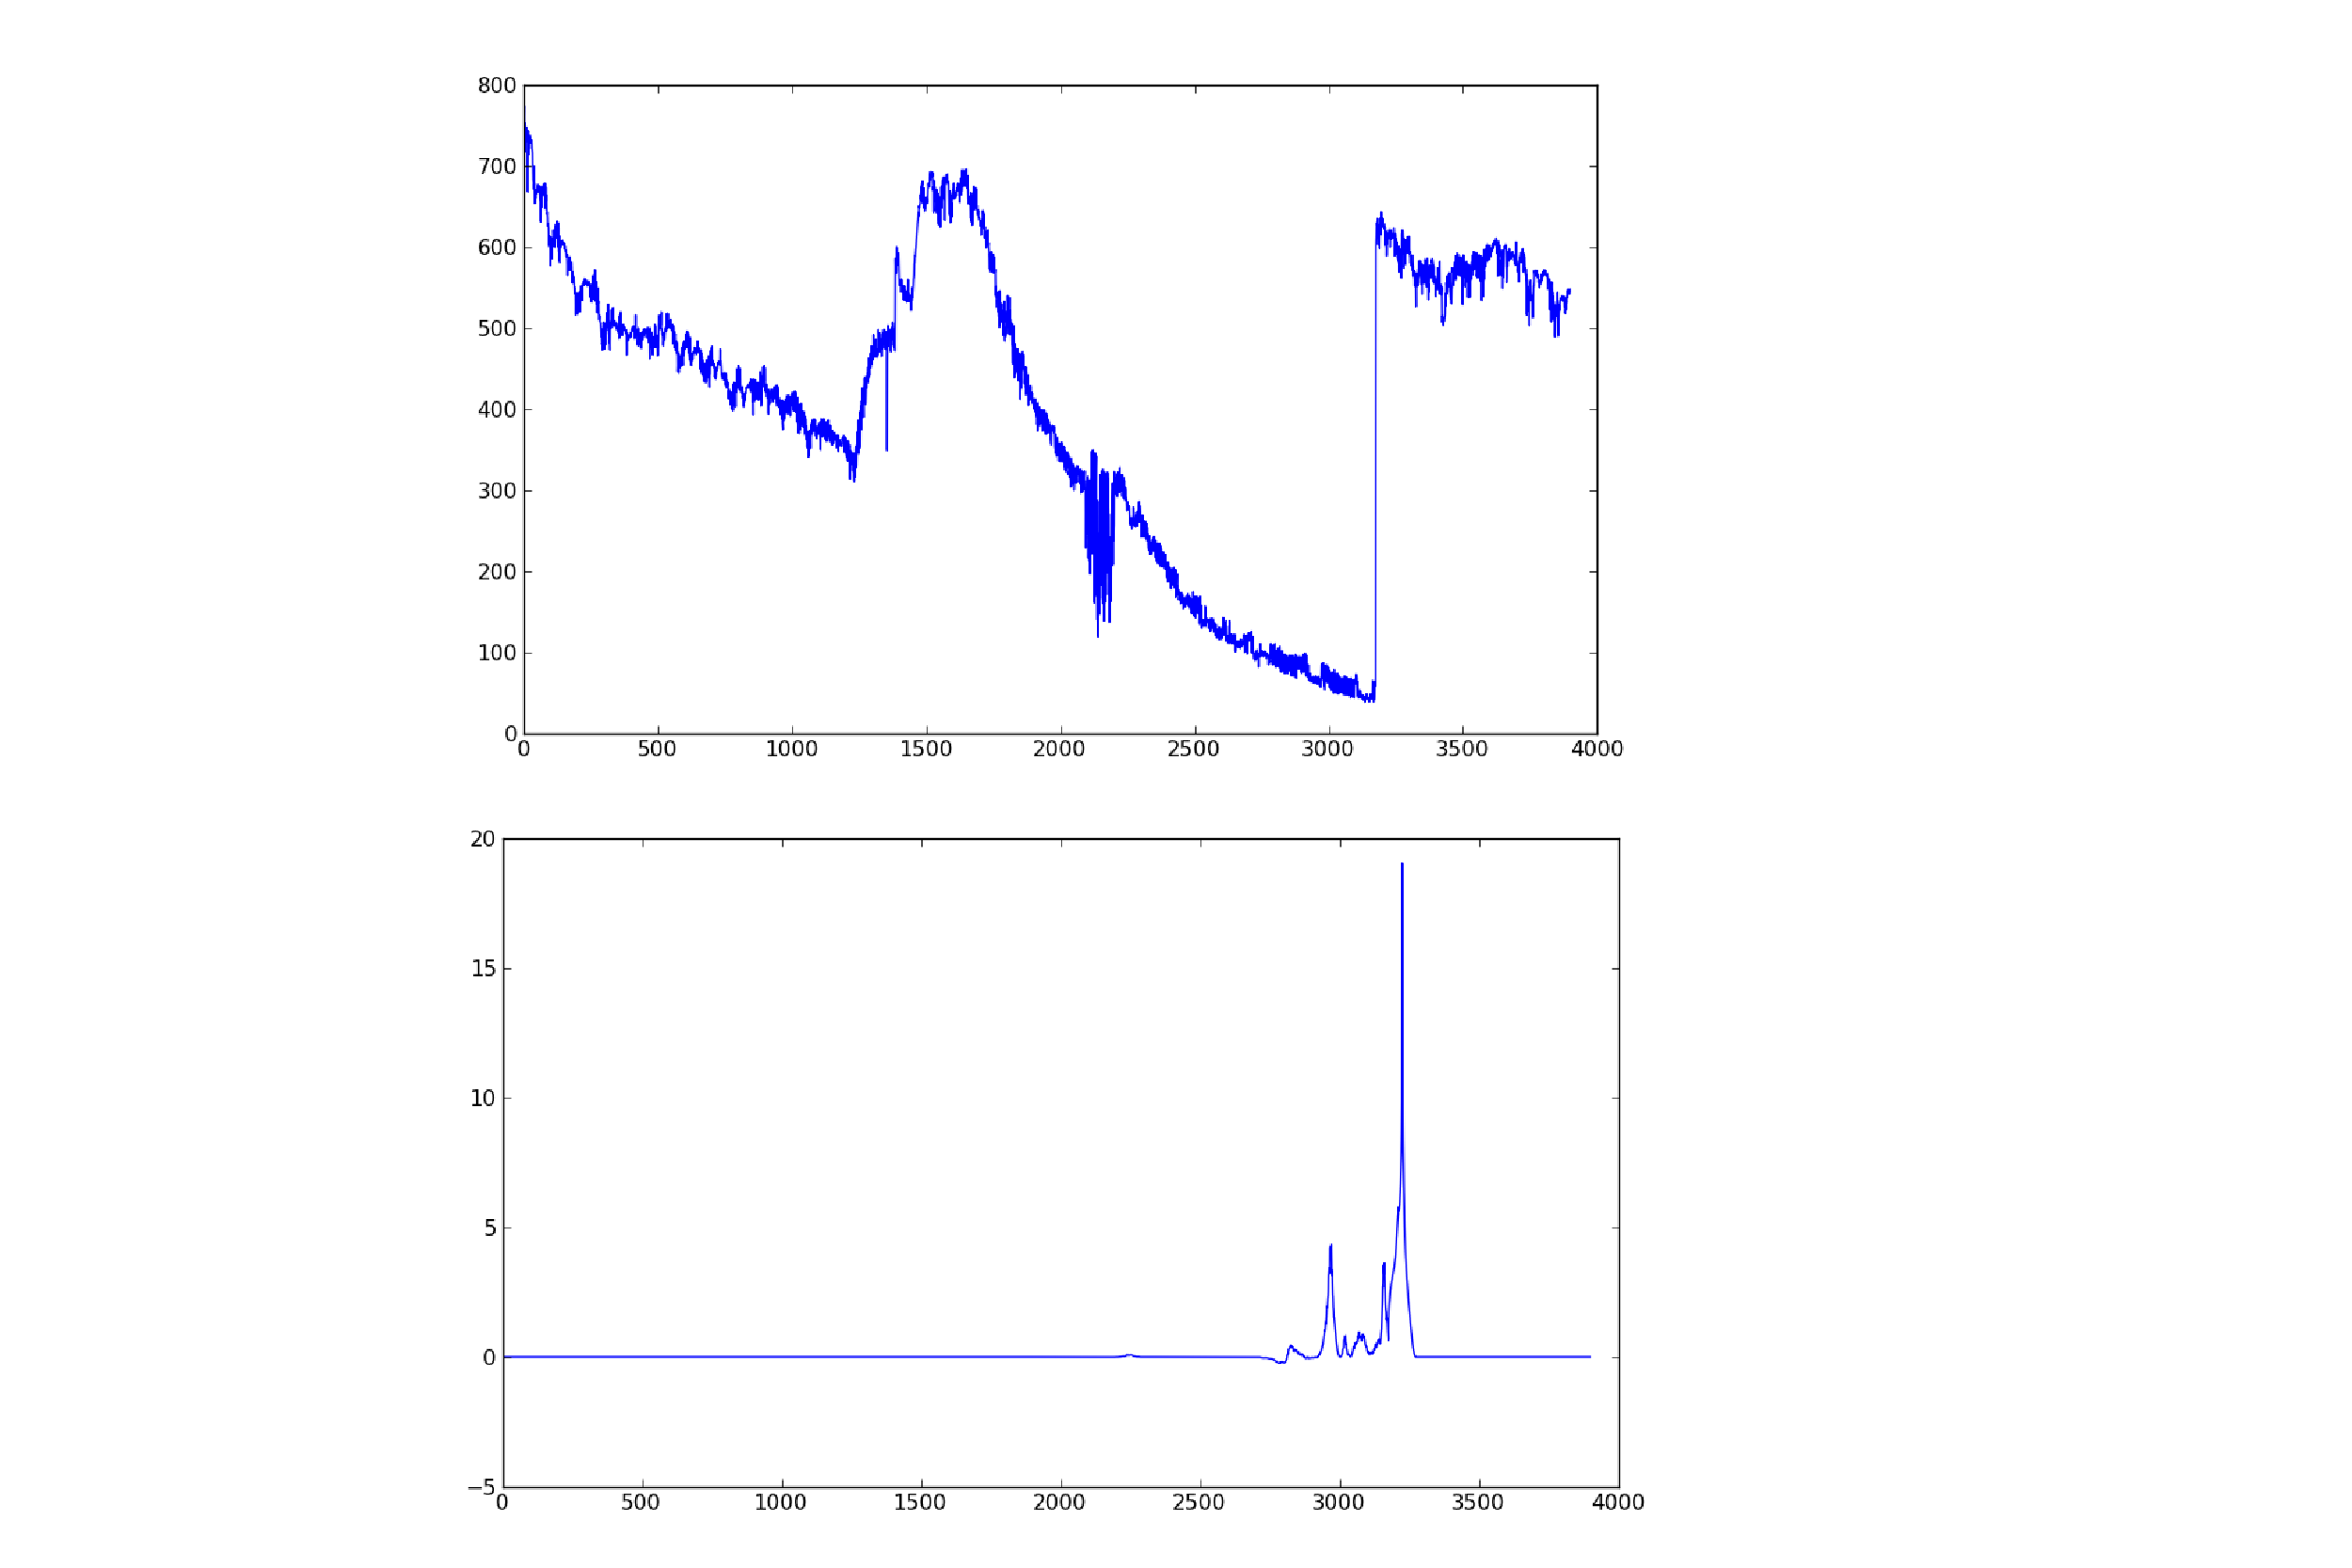
\includegraphics[width=\textwidth]{../../figures/troutlake}
\end{frame}


\section{Future directions}
%So, so many.

\begin{frame}{Future directions}
	Add dependence on other variables (regression):\\
	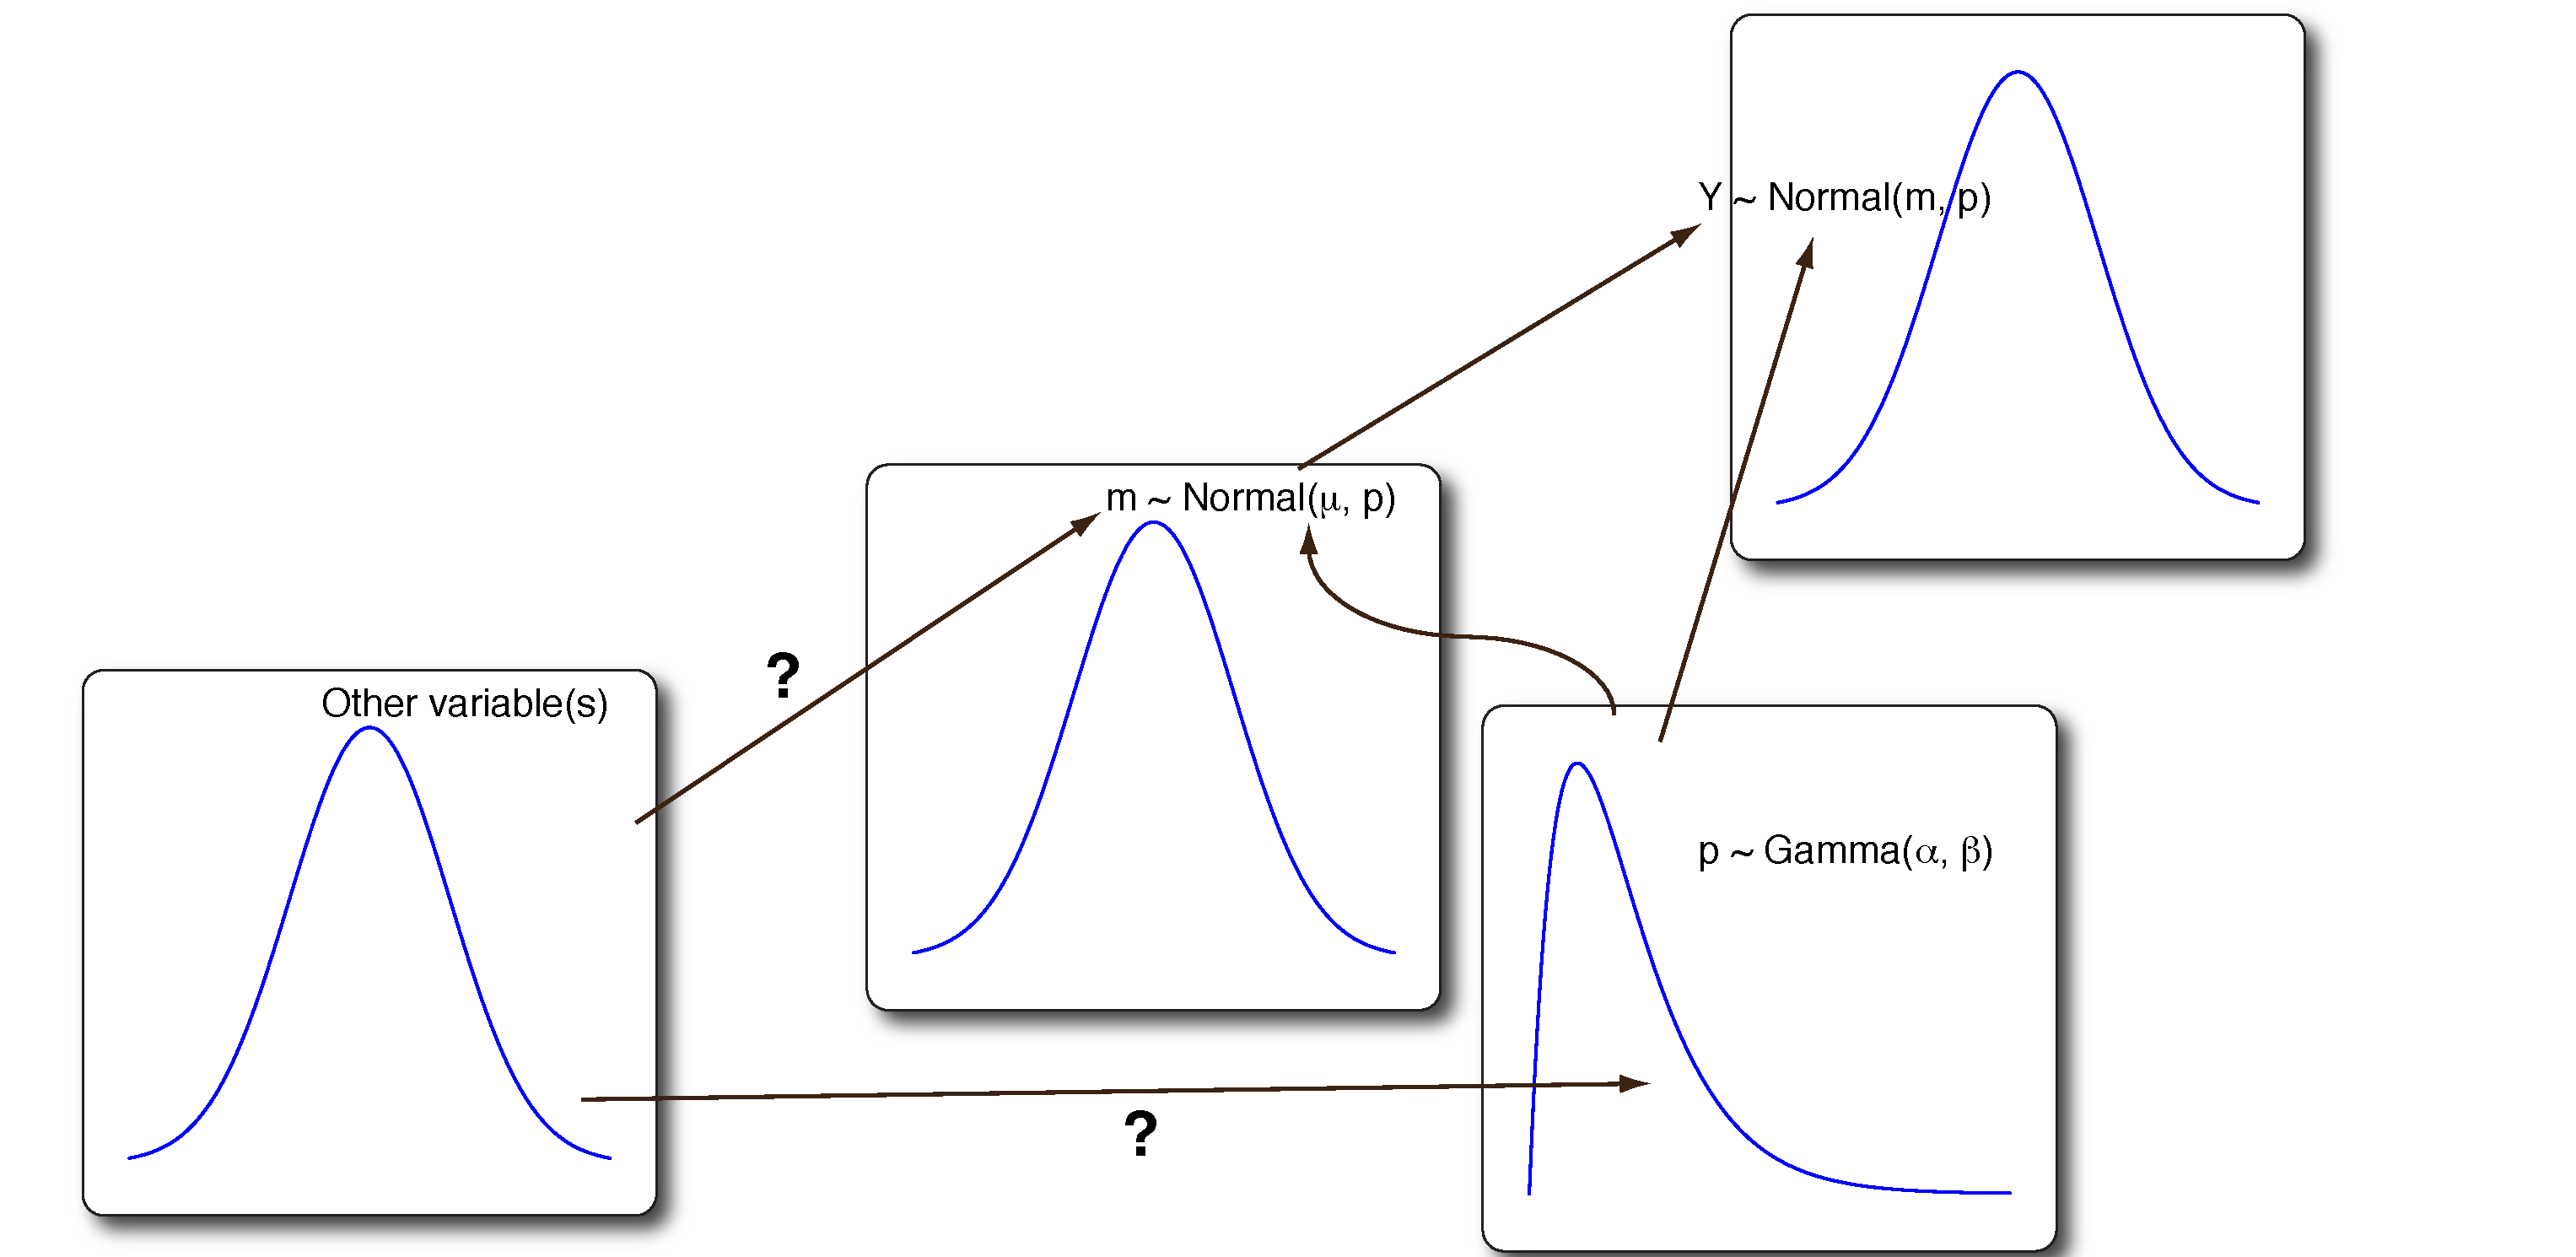
\includegraphics[width=\textwidth]{../../figures/hierarchical-regression}
\end{frame}


\begin{frame}{Conclusion}
	\begin{itemize}
		\item Surprise is a data-driven tool that can help to quickly detect problems with real-time sensors and therefore improve the up-time of a monitoring effort.
	\end{itemize}
\end{frame}


\end{document}